\documentclass[aps,prd,superscriptaddress,nofootinbib,longbibliography,notitlepage,11pt]{revtex4-2}
\usepackage{amsmath,amssymb,bm}
\usepackage{graphicx}
\usepackage{booktabs}
\usepackage{siunitx}
\usepackage{xcolor}
\usepackage[colorlinks=true,linkcolor=blue!60!black,citecolor=blue!60!black,urlcolor=blue!60!black]{hyperref}
\usepackage[capitalize]{cleveref}
\usepackage{caption}
% RevTeX/APS sets captions and tables in \footnotesize/\small by default; make
% everything the same size as the running text.
\captionsetup{font=normalsize,labelfont=bf,skip=6pt}
\graphicspath{{plots/}}
\sisetup{range-phrase=--,range-units=single}

\newcommand{\eves}{E$\nu$ES}
\newcommand{\sw}{\sin^2\theta_W}
\newcommand{\dmee}{\Delta m^2_{ee}}
\newcommand{\dm}[1]{\Delta m^2_{#1}}
\newcommand{\st}[1]{\sin^2 2\theta_{#1}}
\newcommand{\MWyr}{\mathrm{MW\,yr}}

\begin{document}
\title{A compact HALEU reactor parked at JUNO:\\
Standard-Model precision, sterile-neutrino wiggles, and axion-like particles}
\author{Internal report on notebooks 5--7 of the \texttt{JUNO} repository}
\date{\today}
\begin{abstract}
This report summarises what I have done on the physics case for a compact
high-assay low-enriched-uranium (HALEU) research reactor of $10\,\mathrm{MW_{th}}$ parked
about $50$~m from the JUNO central detector.  Three studies are carried out within one
analysis framework, built on the measured Daya Bay antineutrino spectra, JUNO's released
detector response, and analytic Asimov profiling over joint Gaussian nuisance modes.
First, elastic neutrino--electron scattering (\eves) at $\sim3\times10^3$~events per day
gives a $\sim2\%$ determination of the low-energy weak mixing angle when analysed alone
(where the measured flux shape is the limit), and $\sigma(\sw)=1.4\times10^{-3}$
($0.6\%$) when the $6\times10^4$ per day inverse-beta-decay (IBD) sample is used to anchor
the flux in situ, with $8\times10^{-4}$ within reach of plausible transfer systematics.
JUNO's measured detector singles are included ($4.7$~Hz above $0.7$~MeV, overwhelmingly
external $\gamma$ that stop at the $2.615$~MeV $^{208}$Tl line), and running the
reactor off for as long as on measures them in situ, which leaves the answer intact even
if they are thirty times larger than modelled.
Second, for $\dm{41}\sim0.1$--$10\,\mathrm{eV^2}$ the sterile-neutrino oscillation length is
metres, so JUNO's 33~m diameter turns the detector into a many-baseline experiment.  A
shape-only, vertex-binned wiggle search reaches $\st{14}\approx10^{-3}$ over
$0.26$--$1.1\,\mathrm{eV^2}$ and stays below $2\times10^{-3}$ from $0.13$ to
$2.7\,\mathrm{eV^2}$, an order of magnitude beyond the reactor short-baseline programme.
An integrated analysis of the same data with the same free flux shape has no sensitivity
at all, so the finite detector is not an improvement on the conventional analysis but the
only thing that makes a prior-free search possible; the full 3+1 formula is carried across
standoffs of $50$--$1400$~m.  Third, the core's
$\sim5\times10^{18}\,\gamma/\mathrm{s}$ produce axion-like particles (ALPs) through
Primakoff and Compton-like conversion; with an $855\,\mathrm{m^2}$ face and 22~m mean decay
path, JUNO covers the ``cosmological triangle'' of the ALP--photon plane in full and reaches
$g_{aee}\sim10^{-8}$ at MeV masses with the background included.  Every cross section,
decay rate and flux ingredient is validated against independent implementations or analytic
benchmarks, and the systematics budgets and their limitations are stated explicitly.
\end{abstract}
\maketitle
\tableofcontents

%======================================================================
\section{Common framework}
\label{sec:framework}

All three studies share one set of inputs and one statistical machinery, so I describe them once here.

\paragraph{Source and fuel evolution.}
A HALEU core of thermal power $P$ with fission fractions $f_i(\beta)$
($i=\,^{235}$U, $^{238}$U, $^{239}$Pu, $^{241}$Pu; $\sum_if_i=1$) at burnup position
$\beta\in[0,1]$ in its cycle has fission rate and antineutrino flux
\begin{equation}
R_f(\beta)=\frac{P}{\sum_i f_i(\beta)\,E_i},\qquad
\frac{d\Phi_\nu}{dE_\nu}(E_\nu,\beta)=\frac{R_f(\beta)}{4\pi L^2}\sum_i f_i(\beta)\,S_i(E_\nu),
\label{eq:source}
\end{equation}
with the thermal energies per fission $E_i=(202.36,\,205.99,\,211.12,\,214.26)$~MeV
\cite{ParticleDataGroup:2024cfk} and $S_i$ the per-fission antineutrino spectra.  For
$P=10\,\mathrm{MW}$ this gives $R_f=3.07\times10^{17}\,\mathrm{s^{-1}}$ at $\beta=0.5$.
The fresh composition is $f_{235}=0.98$, $f_{238}=0.02$, and plutonium grows in along the
\emph{Daya Bay} fuel-evolution trajectory \cite{DayaBay:2017jkb}: with the measured
$^{239}$Pu and $^{241}$Pu fission fractions $F_{239,241}(\beta_k)$ across Daya Bay's 20
burnup groups ($\beta_k$ mapped linearly onto $[0,1]$),
\begin{equation}
f_{239}(\beta)=F_{239}(\beta)-F_{239}(0),\qquad
f_{241}(\beta)=F_{241}(\beta)-F_{241}(0),\qquad
f_{238}=0.02,\qquad
f_{235}=1-f_{238}-f_{239}-f_{241},
\label{eq:evolution}
\end{equation}
that is, the LEU \emph{increments} of the Pu fractions are applied on top of the fresh HALEU
composition at fixed $^{238}$U.  This is deliberately conservative: a $2\%$-$^{238}$U core
breeds plutonium more slowly than the LEU cores the trajectory describes, so the true
spectral drift is smaller than modelled.  At the run-averaged $\beta=0.5$ used throughout,
$(f_{235},f_{238},f_{239},f_{241})=(0.901,\,0.020,\,0.063,\,0.016)$; at end of cycle
$(0.818,\,0.020,\,0.125,\,0.037)$.  The fuel-evolution \emph{systematic} is a single
nuisance mode scaling the Pu increments by $(1+\epsilon)$, $\sigma_\epsilon=0.30$, whose
spectral direction is
\begin{equation}
\frac{\partial}{\partial\epsilon}\sum_if_iS_i=f_{239}\,(S_{239}-S_{235})+f_{241}\,(S_{241}-S_{235}),
\label{eq:evomode}
\end{equation}
that is, fission share moved from $^{235}$U into plutonium at fixed $^{238}$U.

The per-fission spectra are the \emph{measured} Daya Bay unfolded per-fission IBD yields
for $^{235}$U and $^{239}$Pu \cite{DayaBay:2021dqj}, divided by the Vogel--Beacom cross
section \cite{Vogel:1999zy} wherever a flux rather than a yield is needed, together with
the Huber--Mueller spectra \cite{Huber:2011wv,Mueller:2011nm} for the percent-level
$^{238}$U and $^{241}$Pu components (\cref{app:flux}).  This flux is defined only above
the IBD threshold of 1.806~MeV, so recoil spectra below $T\sim1.5$~MeV are conservative.

\paragraph{Detector.}
I take JUNO's fiducial target to be $N_p=1.44\times10^{33}$ free protons
\cite{JUNO:2025gmd,JUNO:2021vlw}, inside a fiducial radius of $16.5$~m.  That number is
fixed by the delivered scintillator's hydrogen mass fraction of $12.01\%$, and the same
composition fixes the electron count: $\mathrm{H/C}=1.63$ by number, so one carbon comes
with $1.63$ free protons and $7.63$ electrons and $N_e=4.689N_p=6.76\times10^{33}$.  Both
target counts are derived from that one composition rather than quoted separately, because
the joint fit of \cref{sec:sm} measures the \eves/IBD rate ratio and $N_e/N_p$ enters its
answer directly.  The
response uses the released positron and electron non-linearities, an energy resolution
$\sigma_E/E=\sqrt{a^2/E+b^2}$ with $a=3.3\%$ and $b=1.0\%$, a vertex resolution of
$10\,\mathrm{cm}/\sqrt{E}$, a selection efficiency of $0.8$, and a reactor duty cycle of
$0.9$.

\subsection{Statistics}
\label{sec:stats}
Every sensitivity in this report is an Asimov projection \cite{Cowan:2010js}, and since the
same construction is used in all four studies it is worth writing out once.

Let $\bm\theta$ be the physics parameters and $\bm\xi$ a set of nuisance parameters, each
normalised so that it carries a unit Gaussian prior.  The predicted mean in bin $i$ is
$\mu_i(\bm\theta,\bm\xi)$, and the likelihood is the Poisson term for the data plus the
prior term for the pulls,
\begin{equation}
\chi^2(\bm\theta,\bm\xi)=\sum_i\frac{\big[n_i-\mu_i(\bm\theta,\bm\xi)\big]^2}{\mu_i}
+\sum_k\xi_k^2 .
\label{eq:chi2pull}
\end{equation}
Each systematic acts on the prediction through a template, and since the pulls are small by
construction we keep only the linear response,
\begin{equation}
\mu_i(\bm\theta,\bm\xi)\simeq\mu_i(\bm\theta)+\sum_k\xi_k v_{ki},
\qquad
v_{ki}\equiv\frac{\partial\mu_i}{\partial\xi_k}\bigg|_{\bm\xi=0},
\label{eq:modes}
\end{equation}
so $v_k$ is simply the shift in the predicted spectrum produced by moving systematic $k$ by
one standard deviation.  Building the $v_k$ is the whole modelling effort; everything after
that is linear algebra.

Profiling \cref{eq:chi2pull} over $\bm\xi$ is then a Gaussian integral, and the result is
the familiar statement that pull terms and a covariance matrix are two descriptions of the
same thing.  Writing $D=\mathrm{diag}(\mu)$ and $\bm\Delta=\bm n-\bm\mu(\bm\theta)$, and
minimising over $\bm\xi$,
\begin{equation}
\chi^2_{\min}(\bm\theta)=\bm\Delta^{T}C^{-1}\bm\Delta,
\qquad
C=D+\sum_k v_kv_k^{T}=D+V^{T}V,
\label{eq:cov}
\end{equation}
where $V$ is the matrix whose rows are the $v_k$.  The Poisson variance sits on the
diagonal and every systematic adds a rank-one outer product; correlations between bins are
carried entirely by the shapes of the $v_k$.  No nuisance is ever minimised numerically.

For a projection we set the data equal to the prediction at the true point,
$\bm n=\bm\mu(\bm\theta_0)$, which is what makes it an Asimov dataset.  Expanding
$\bm\mu(\bm\theta)$ to first order about $\bm\theta_0$ turns \cref{eq:cov} into a quadratic
form,
\begin{equation}
\Delta\chi^2(\bm\theta)=(\bm\theta-\bm\theta_0)^{T}F\,(\bm\theta-\bm\theta_0),
\qquad
F_{ab}=\Big(\frac{\partial\bm\mu}{\partial\theta_a}\Big)^{T}C^{-1}
\Big(\frac{\partial\bm\mu}{\partial\theta_b}\Big),
\label{eq:fisher}
\end{equation}
so the projected uncertainty on one parameter with all others profiled is
$\sigma(\theta_a)=\sqrt{(F^{-1})_{aa}}$, and for a single parameter alone
$\sigma(\theta)=1/\sqrt{\bm d^{T}C^{-1}\bm d}$ with $\bm d=\partial\bm\mu/\partial\theta$.
This is the expression evaluated for $\sw$ and for $(g_V,g_A)$ in \cref{sec:sm}.

Two practical points make it cheap.  First, $C$ is a diagonal matrix plus a low-rank
correction, so the Woodbury identity
\begin{equation}
C^{-1}=D^{-1}-D^{-1}V^{T}\big(\mathbb{1}+VD^{-1}V^{T}\big)^{-1}VD^{-1}
\label{eq:woodbury}
\end{equation}
replaces the inversion of an $N_{\rm bins}\times N_{\rm bins}$ matrix by that of an
$N_{\rm modes}\times N_{\rm modes}$ one.  With $50$~keV binning and a few tens of modes this
is the difference between a scan that runs in seconds and one that does not run at all, and
it is what allows the sterile analysis of \cref{sec:sterile} to leave one unconstrained mode
free per energy bin.  Second, whenever the prediction is affine in a parameter, as it is in
the couplings and in $\st{14}$, the templates are built once and every point of a scan is an
algebraic combination of them rather than a re-evaluation of the physics.

\subsection{When does the near reactor pile up?}
\label{sec:pileup}
A reactor at tens of metres produces IBD at roughly $1$~Hz per $10\,\mathrm{MW}$
($R_{\rm IBD}=0.69\,\mathrm{Hz}$ at $10\,\mathrm{MW}$ and $50$~m, scaling as $P/D^2$), each
event being a prompt hit followed by a delayed neutron capture about $200\,\mu$s later.
Three distinct pile-up questions arise, and they have very different thresholds.

\emph{(i) Accidental IBD-like coincidences.}  JUNO's measured fiducial singles above
$0.7$~MeV run at $R_{\rm sing}=4.7$~Hz \cite{JUNO:2026ixk} (\cref{sec:singles}), and the
reactor adds delayed neutron captures at $R_{\rm IBD}$.  A random pairing of one of each
inside the coincidence window $\tau$ and the $1.5$~m distance cut is an accidental IBD
candidate, at a rate
\begin{equation}
R_{\rm acc}\simeq R_{\rm sing}\,R_{\rm IBD}\,\tau\,f_{\rm vol},
\qquad f_{\rm vol}\sim\Big(\frac{1.5\ \mathrm{m}}{R_{\rm fid}}\Big)^{3},
\label{eq:accidental}
\end{equation}
Both $R_{\rm acc}$ and the true rate $R_{\rm IBD}$ scale linearly with reactor power, so
their ratio,
\begin{equation}
\frac{R_{\rm acc}}{R_{\rm IBD}}\simeq R_{\rm sing}\,\tau\,f_{\rm vol},
\label{eq:accratio}
\end{equation}
is independent of power and distance altogether and is fixed by JUNO's own singles rate
rather than by the source.  With $\tau=1$~ms and $R_{\rm fid}=16.5$~m this is
$3.5\times10^{-6}$: $0.21$ against $6.0\times10^4$ events per day at $10\,\mathrm{MW}$ and
$50$~m.  Note that this is a different mechanism from the accidentals JUNO already
subtracts, which pair two \emph{singles} ($0.049$ per day in the 59-day release
\cite{JUNO:2025gmd}) and do not scale with any reactor at all; the near reactor adds a
term that is negligible next to it.  Either way this is a background one \emph{measures}
from off-window sidebands, not a pile-up limit.

\emph{(ii) Genuine IBD self-pile-up.}  Two reactor IBDs within one coincidence window
($\tau\sim1$~ms) confuse the prompt-to-delayed pairing.  Since the events are Poisson in
time, the probability that a given IBD is accompanied by at least one more within $\tau$ is
\begin{equation}
P_{\rm pile}=1-e^{-R_{\rm IBD}\tau}\simeq R_{\rm IBD}\,\tau
\qquad(R_{\rm IBD}\tau\ll1),
\label{eq:selfpile}
\end{equation}
and this one does \emph{not} cancel: it grows linearly with the source.  Numerically it is
$7\times10^{-4}$ at $10\,\mathrm{MW}$ and $50$~m, $0.7\%$ at $100\,\mathrm{MW}$, and $6.7\%$
at $1\,\mathrm{GW}$.  This is therefore the operative boundary.  Writing
$R_{\rm IBD}\propto P/D^{2}$ and imposing $P_{\rm pile}<1\%$ gives a condition on the source
strength alone,
\begin{equation}
    \frac{P}{D^2}\lesssim 0.06\,\mathrm{MW\,m^{-2}}, \qquad\text{i.e.}\qquad
    P\lesssim 150\,\mathrm{MW}\left(\frac{D}{50\,\mathrm{m}}\right)^2,
\label{eq:pileup}
\end{equation}
which corresponds to $\approx8.6\times10^5$ IBD per day whatever the geometry
($145\,\mathrm{MW}$ at $50$~m, $580\,\mathrm{MW}$ at $100$~m, $2.3\,\mathrm{GW}$ at $200$~m).
Every configuration in this report ($10\,\mathrm{MW}$ at $50$~m, and up to $100\,\mathrm{MW}$
in the mobile-reactor study of notebook~2) sits comfortably inside it; a GW-class core would
have to stand $\gtrsim150$~m away.

\emph{(iii) Single-hit dead time and DAQ.}  The reactor's total hit rate (prompt, delayed
and \eves) is $1.4$~Hz at $10\,\mathrm{MW}$ and $50$~m, and only $145$~Hz even at
$1\,\mathrm{GW}$ and $50$~m, which is $0.01\%$ to $1.5\%$ of the radioactivity singles JUNO
already triggers on.  Event overlap within a $\sim1\,\mu$s readout window stays at the
$\sim1\%$ level set by radioactivity, independent of the reactor.  Single-hit physics is
therefore never rate-limited by the reactor; its reactor-induced backgrounds are the
\emph{untagged} IBD positrons and the \eves{} events themselves, which are modelled
explicitly in \cref{sec:sm,sec:sterile,sec:alps}.  (The reactor's own neutrons and gammas
leaking through its shield are a separate, shielding-design question addressed in
notebook~8; see \cref{sec:discussion}.)

The conclusion is that below the boundary of \cref{eq:pileup} pile-up is a percent-level
nuisance measured in situ, and the physics reach is set by statistics and systematics, not
by rate.

%======================================================================
\section{Standard-Model precision with \eves{} (notebook 5)}
\label{sec:sm}

\subsection{Cross sections and rates}
The observable is elastic scattering off atomic electrons, so it is worth setting up the
couplings carefully: the whole measurement is a statement about them.  Below the $W$ and
$Z$ masses the interaction is a four-fermion contact term, and for
$\nu_\alpha e\to\nu_\alpha e$ two diagrams contribute.  Every flavour has the neutral
current,
\begin{equation}
\mathcal{L}_{\rm NC}=-\frac{G_F}{\sqrt2}
\big[\bar\nu_\alpha\gamma^\mu(1-\gamma_5)\nu_\alpha\big]
\big[\bar e\gamma_\mu(g_V-g_A\gamma_5)e\big],
\qquad g_V=2\sw-\tfrac12,\quad g_A=-\tfrac12 ,
\label{eq:lnc_eves}
\end{equation}
while for $\alpha=e$ alone there is in addition the charged current, in which the
$W$ is exchanged between the $\nu_e$ and the electron.  A Fierz rearrangement turns that
charged-current term into the same $(V-A)\times(V-A)$ structure as \cref{eq:lnc_eves} with
unit couplings, so the two simply add and the effect of the charged current is the shift
\begin{equation}
C_V=g_V+\delta_{\alpha e},\qquad C_A=g_A+\delta_{\alpha e} .
\label{eq:cvca}
\end{equation}
This is why $\nu_e$ and $\bar\nu_e$ scatter so differently from $\nu_{\mu,\tau}$, and why a
reactor experiment measuring $\bar\nu_e e$ is sensitive to a combination of couplings
different from the one an accelerator $\nu_\mu e$ experiment measures.

It is convenient to move to chiral couplings, $C_{L,R}=\tfrac12(C_V\pm C_A)$ for neutrinos,
because then the two helicity configurations contribute incoherently and the differential
cross section takes its standard form.  For antineutrinos the roles of $L$ and $R$
interchange, $C_{L,R}=\tfrac12(C_V\mp C_A)$, and
\begin{equation}
\frac{d\sigma}{dT}=\frac{2G_F^2m_e}{\pi}\Big[C_L^2+C_R^2\Big(1-\frac{T}{E}\Big)^2
-C_LC_R\frac{m_eT}{E^2}\Big].
\label{eq:dsdT}
\end{equation}
The three terms have clean interpretations.  The first is helicity-conserving scattering,
isotropic in the centre of mass and therefore flat in $T$.  The second is
helicity-flipping, suppressed by the $(1-T/E)^2$ factor that vanishes at the kinematic
endpoint.  The third is the interference of the two, suppressed by $m_eT/E^2$ and
negligible at reactor energies.  The kinematic limit follows from two-body kinematics,
\begin{equation}
T_{\max}=\frac{2E^2}{m_e+2E},
\label{eq:tmax}
\end{equation}
which for $E=4$~MeV gives $T_{\max}=3.76$~MeV: the recoil takes almost the whole neutrino
energy, so the $T>1$~MeV analysis window would reach down to $E_\nu=1.21$~MeV, below the
IBD threshold at which the measured flux stops.  The reference point used throughout is the PDG 2024 world average of the $\nu$--$e$ couplings, $g_V=-0.040$ and
$g_A=-0.507$ \cite{ParticleDataGroup:2024cfk}, which coincides with the radiatively
corrected SM prediction ($-0.0395$, $-0.5063$ \cite{Erler:2004in}) and corresponds to an
effective low-energy $\sw=(g_V+\tfrac12)/2=0.230$; sensitivities are quoted as errors on
that effective $\sw$.  Cross sections come from \textsc{Neptune} \cite{NEPTUNE}, and the
parametric $(g_V,g_A)$ implementation used for the scans reproduces its recoil shape to
machine precision at \textsc{Neptune}'s own tree-level couplings ($\sw=0.2223$,
$g_A=-\tfrac12$).  The absolute normalisation uses
$(\hbar c)^2=3.8938\times10^{-28}\,\mathrm{GeV^2\,cm^2}$: a shift of this constant is a
shift of the \eves{} rate, and under the IBD anchor of \cref{sec:results} a $0.7\%$ one
would move $\sw$ by $1.4\times10^{-3}$, which is the whole error budget.  \Cref{fig:xsec} compares the cross sections per carbon of LAB, and
\cref{fig:dsdt} shows the recoil shapes at fixed $E_\nu$.  The unit is the CH$_{1.63}$ of
\cref{sec:framework}: one carbon nucleus, $1.63$ free protons and $7.63$ electrons.  (I also evaluated the trident channel $\bar\nu_eN\to\bar\nu_ee^+e^-N$ with
\textsc{Neptune}, coherently on carbon and elastically on the free protons: at reactor
energies it is $O(\alpha)$ and phase-space suppressed above its $1.02$~MeV threshold and
amounts to $\sim10^{-5}$ of the \eves{} rate, $0.04$ events per day at $10\,\mathrm{MW}$
and 50~m, so it is not carried further.)  Four features drive the analysis.  IBD is $\sim100\times$ larger per
molecule than $\bar\nu_e e$ even after the $7.63$ electrons are counted, which is why the
IBD sample is $20\times$ the \eves{} one.  The antineutrino cross section lies \emph{below} the neutrino one for two reasons that
are worth keeping apart.  The charged current shifts $C_V$ and $C_A$ by the same $+1$, so
it enhances the flat $C_L^2$ term for $\nu_e$ but the phase-space-suppressed
$C_R^2(1-T/E)^2$ term for $\bar\nu_e$, whose flat coupling
$C_L=\tfrac12(C_V-C_A)=\sw$ is left untouched and is small.  On top of that the CC--NC
interference is genuinely destructive for $\bar\nu_e$: adding the pure-NC and pure-CC
rates would give $0.412$ in units where the full answer is $0.231$.  The NC-only $\bar\nu_{\mu,\tau}$ channel is a
further factor $\sim3$ down; it is irrelevant at 50~m but carried anyway.  And the $T>1$~MeV
window removes about $60\%$ of the $\bar\nu_e e$ rate at $E_\nu=3$~MeV, less at higher
energy.  The $\bar\nu_e$ recoil spectrum is flat and then falls in $T$ (the $C_R^2(1-T/E)^2$
term), and it is the $E_\nu$-dependence of that fall-off, not the total rate, that carries
the $\sw$ information once the normalisation is free.

\begin{figure}[t]\centering
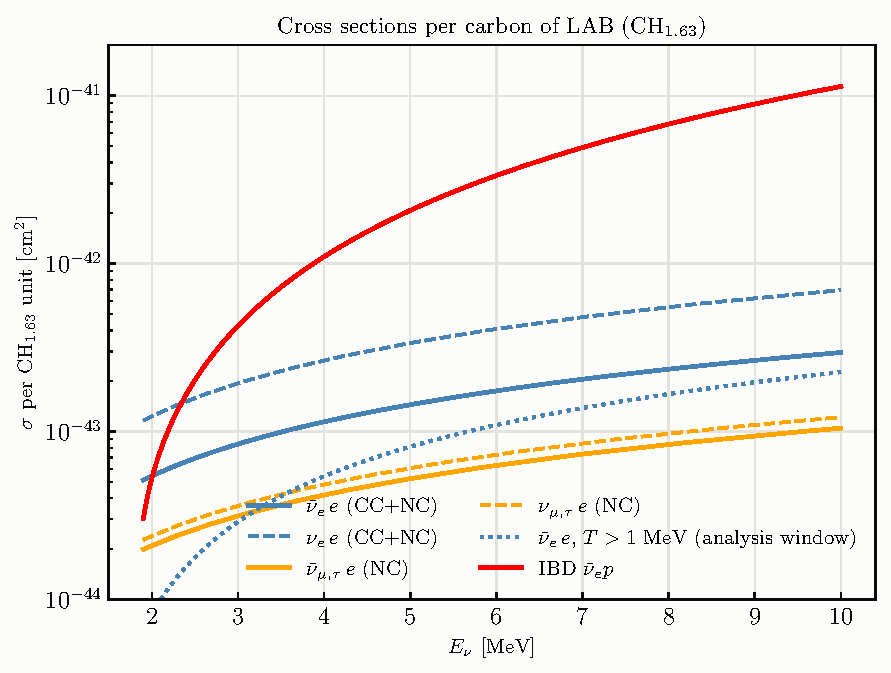
\includegraphics[width=\textwidth]{nb5_cross_sections}
\caption{Cross sections per carbon of LAB (one CH$_{1.63}$ unit: 1 carbon, 1.63
free protons, 7.63 electrons): \eves{} for $\bar\nu_e$/$\nu_e$ (CC+NC) and
$\bar\nu_{\mu,\tau}$/$\nu_{\mu,\tau}$ (NC), the $\bar\nu_e e$ rate restricted to the
$T>1$~MeV analysis window, and IBD on the free protons \cite{Vogel:1999zy}.}
\label{fig:xsec}
\end{figure}
\begin{figure}[t]\centering
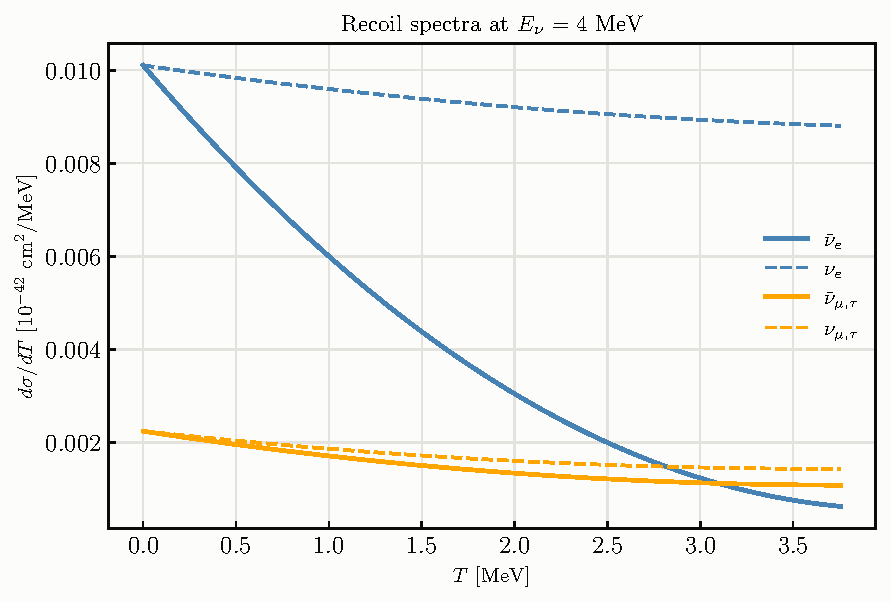
\includegraphics[width=\textwidth]{nb5_dsigma_dT}
\caption{Recoil spectra $d\sigma/dT$ at $E_\nu=4$~MeV for the four flavour/helicity
channels; the antineutrino--neutrino difference is the CC--NC interference.}
\label{fig:dsdt}
\end{figure}

The flavour composition is exact at every baseline, here and in \cref{sec:sterile}: the
$\bar\nu_{\mu,\tau}$ component from $1-P_{ee}$ ($6\times10^{-4}$ at 50~m, $6\%$ at
$1.4$~km) is carried with its NC-only cross section.  An electron only
participates for $T$ above its binding energy (carbon K~284~eV, L~19/11~eV, hydrogen
13.6~eV); this atomic-binding correction \cite{Kopeikin:2003bx} is applied to every
spectrum and is exactly unity above 1~keV, so it is completely negligible for the analysis
window $T\in[1,6.5]$~MeV.

The resulting rates for $10\,\mathrm{MW}$ at $50$~m are $5.95\times10^4$ IBD per day
($\sim1700\times$ the far reactors) and $3.2\times10^3$ \eves{} per day in the analysis
window, $99.99\%$ of them $\bar\nu_e$.  Because the flux stops at the IBD threshold and
$T_{\max}(1.806\,\mathrm{MeV})=1.58$~MeV, $48\%$ of that \eves{} rate sits in a part of the
window the flux model cannot fill; the quoted rate is therefore a lower bound there, and
the model carries an artificial edge at $1.58$~MeV.  It costs nothing: closing the window
at $T>1.6$~MeV instead of $T>1$~MeV moves $\sigma(\sw)$ from $0.137$ to $0.138$, because
what the joint fit measures is a rate ratio in which both channels share the same flux.
\Cref{fig:eves_fake} shows the recoil spectrum with the backgrounds I model: IBD singles
(untagged-neutron fraction $1\%$, $577$ per day, measurable in situ from the $99\%$-tagged
sample), solar neutrinos ($^8$B, hep and CNO continua plus the pep line
\cite{Bahcall:1996qv,Vinyoles:2016djt}, LMA flavour-weighted, 164 per calendar day), and
the detector's own singles, which dominate everything else and are the subject of
\cref{sec:singles}.

\begin{figure}[t]\centering
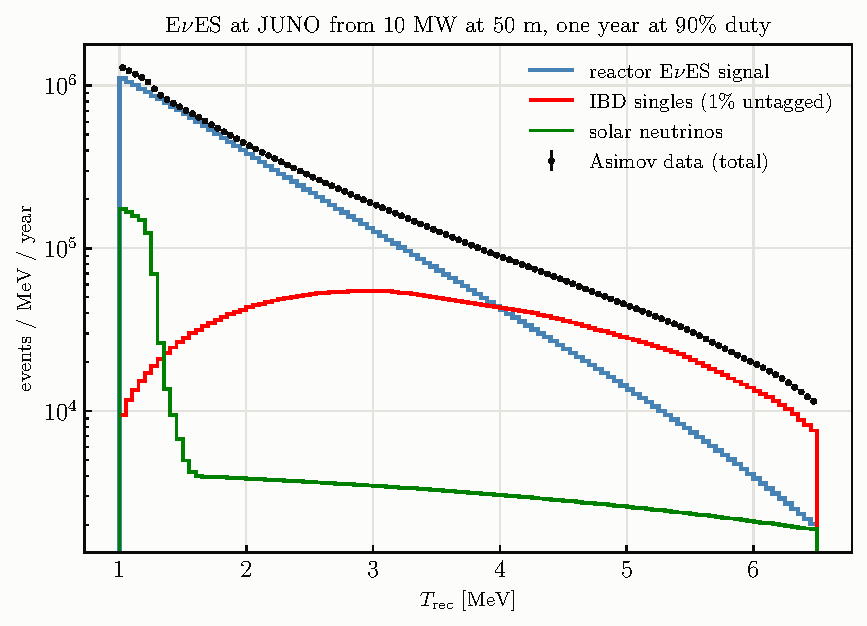
\includegraphics[width=\textwidth]{nb5_eves_fake_data}
\caption{Asimov \eves{} recoil spectrum with the modelled backgrounds, per calendar year
at $90\%$ duty, for $10\,\mathrm{MW}$ at $50$~m ($\approx1.1\times10^6$ signal,
$1.9\times10^5$ IBD singles, $6\times10^4$ solar, $4.5\times10^7$ detector-singles and
$1.4\times10^3$ $^{13}$C NC events per year in the window).}
\label{fig:eves_fake}
\end{figure}

\subsection{Detector singles, and the reactor-off measurement}
\label{sec:singles}
The dominant single-hit background is not the reactor but JUNO itself, and two recent
measurements pin it down.  The final radioactivity assessment \cite{JUNO:2026ixk}
reports, from first data, a fiducial singles rate of $4.7$~Hz above $0.7$~MeV for
$R<17.2$~m, better than the $7.2$~Hz design budget.  The delivered scintillator has
U/Th $\lesssim3.4\times10^{-17}$~g/g, some $30\times$ purer than the $10^{-15}$
requirement, so the internal component collapses to $\lesssim0.1$~Hz and \emph{$\sim95\%$
of the fiducial singles are external $\gamma$} from the acrylic vessel, the PMT glass and
the steel truss.  On the solar side \cite{Gavrikov:2025rlg} the same backgrounds set
JUNO's own $^8$B threshold at 2~MeV, through cosmogenic $^{11}$C.

The spectral consequence is what makes the measurement possible (\cref{fig:singles}).  An
external $\gamma$ can deposit at most its own line energy, so the external component
\emph{stops at the $2.615$~MeV $^{208}$Tl line}.  An internal decay contains its whole
cascade, so internal $^{208}$Tl reaches $5.0$~MeV, but only at $\sim84$ decays per day
in 20~kt at the measured purity.  Across the $2.6$~MeV wall the singles fall by three
orders of magnitude, from $3.6\times10^4$ per day in $2$--$3$~MeV to $26$ per day in
$3$--$4$~MeV, and the signal-to-background turns over from $0.02$ to $9$.

\begin{figure}[t]\centering
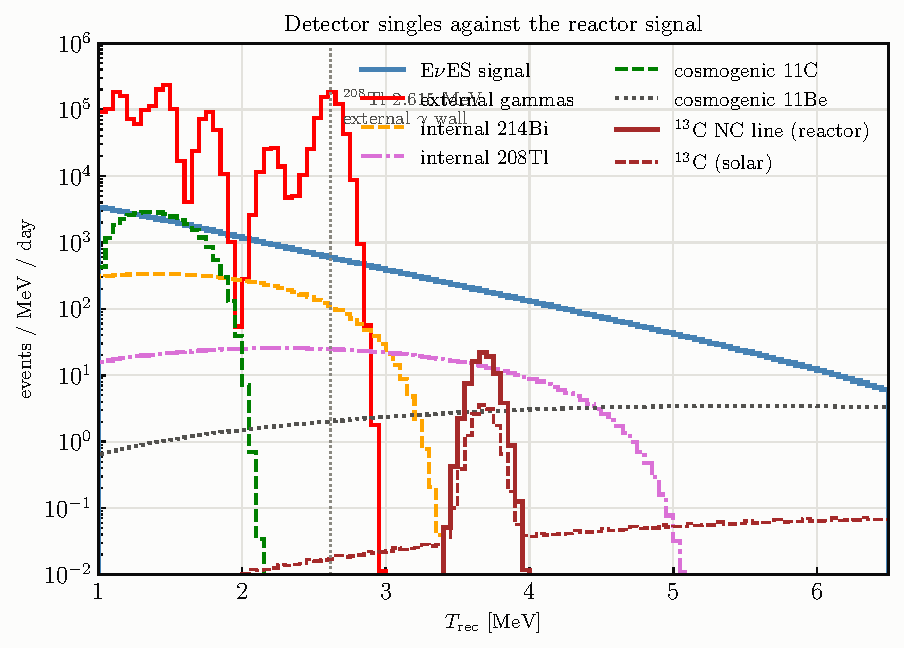
\includegraphics[width=\textwidth]{nb5_singles}
\caption{Detector singles by component against the \eves{} signal at $R=16.5$~m.  The
external $\gamma$ component ends at the $^{208}$Tl line; above it only internal $^{208}$Tl
(full $5.0$~MeV cascade), the cosmogenics and the $^{13}$C lines survive.  The
reactor-driven $^{13}$C NC line at $3.685$~MeV clears the wall by a megaelectronvolt.}
\label{fig:singles}
\end{figure}

I model this in \texttt{reactor/singles.py}: external $\gamma$ from a composite line list
with Compton continua, internal decays from the \emph{measured} concentrations (so
$^{214}$Bi runs at $\sim730$ and $^{208}$Tl at $\sim84$ per day in 20~kt), and the
cosmogenic isotopes $^{11}$C, $^{10}$C, $^{11}$Be, $^{12}$B, $^{6}$He, $^{8}$Li and
$^{9}$Li with a JUNO-like veto suite.  The \emph{rate} is anchored to the measurement, but
the \emph{shape} is a component model rather than a transport simulation, the radial
profile is an effective exponential tuned to their Fig.~6 rather than a $\gamma$
attenuation length (their own reconstruction systematic on the FV singles is
$20$--$30\%$), and the cosmogenic rates are depth-scaled estimates good to a factor of a
few.  These numbers should not be taken at face value, so the analysis is built not to
depend on them.

\paragraph{Turning the reactor off.}
A parked research reactor can be switched off; the singles cannot.  A reactor-off run
therefore measures the entire non-reactor background in situ, bin by bin, with no model at
all, and it is worth working through what that is worth, because the answer is what protects
everything above from the provisional rates.

Take one bin and split the reactor-on prediction into three pieces: the signal $S$, the
reactor-correlated background $R$ (the untagged IBD positrons), and the non-reactor
background $B$ (singles, solar, and the solar $^{13}$C of \cref{sec:c13}).  Running for a
time $t$ with the reactor on and $rt$ with it off gives two measurements,
\begin{equation}
\langle N^{\rm on}\rangle=(S+R+B)\,t,
\qquad
\langle N^{\rm off}\rangle=B\,rt,
\label{eq:onoffmeans}
\end{equation}
and we now treat $B$ as a completely free parameter, one per bin, with no prior whatsoever.
That is the crucial modelling choice.  We are not assuming the singles level, and we are not
assuming their spectral shape either, since a free normalisation in every bin subsumes any
distortion one could write down.

Let $\delta$ be a shift of $B$ away from its nominal value.  It moves the on-prediction by
$\delta t$ and the off-prediction by $\delta rt$, so with $x$ and $y$ the residuals of the
two measurements and $V_{\rm on}=(S+R+B)t$, $V_{\rm off}=Brt$ their variances,
\begin{equation}
\chi^2(\delta)=\frac{(x-\delta t)^2}{V_{\rm on}}+\frac{(y-\delta rt)^2}{V_{\rm off}} .
\label{eq:onoffchi2}
\end{equation}
Setting $\partial\chi^2/\partial\delta=0$ gives
\begin{equation}
\hat\delta\,t=\frac{x/V_{\rm on}+r\,y/V_{\rm off}}{1/V_{\rm on}+r^{2}/V_{\rm off}},
\label{eq:deltahat}
\end{equation}
and substituting back collapses the two terms into one,
\begin{equation}
\chi^2_{\min}=\frac{\big(x-y/r\big)^2}{V_{\rm on}+V_{\rm off}/r^{2}} .
\label{eq:onoffprofiled}
\end{equation}
The numerator is exactly the subtracted estimator one would have written down by hand, the
off-sample scaled by $1/r$ to match the on-exposure, and the denominator is its variance.
Writing that variance out,
\begin{equation}
V_{\rm on}+\frac{V_{\rm off}}{r^{2}}
=(S+R+B)\,t+\frac{B\,rt}{r^{2}}
=\Big[S+R+B\Big(1+\frac1r\Big)\Big]t .
\label{eq:onoff}
\end{equation}
So profiling a free per-bin background is not merely tractable, it is a one-line change to
the analysis: every background normalisation systematic disappears and the Poisson term is
inflated by $B/r$.  That is how it is implemented, as an inflation of the diagonal $D$ in
\cref{eq:cov} rather than as $N_{\rm bins}$ extra modes, which keeps $C$ numerically well
conditioned even when $B$ exceeds $S$ by two orders of magnitude.

Three things follow directly from \cref{eq:onoff}.  Equal on and off exposure, $r=1$, gives
the familiar factor of two, $\mathrm{Var}=S+R+2B$.  The result depends on the singles only
through $\sqrt{B}$, never through their assumed level or shape, which is exactly the
protection needed given how provisional those rates are.  And the limit $r\to0$ diverges,
as it must: with no off-sample and a free background in every bin, the signal is perfectly
degenerate with $B$ and there is no measurement at all.  A short off-run is therefore
worse than none: it inflates the variance by $B/r$ while buying almost no sample, and a
$2\%$-length off-run costs $45\%$ on the joint fit.  ``No off-run'' is a different
analysis rather than the $r\to0$ limit of this one --- there the singles \emph{shape}
comes from the model of \cref{sec:singles} and only its normalisation is profiled, which
gives $0.135$ against $0.137$ at $r=1$ --- and any number quoted that way is a statement
about how far one trusts a background simulation, not a statement about data.

The price of $r=1$ is calendar time, since half the wall clock is spent with the reactor
off and a given $\MWyr$ takes twice as long to deliver.  That is also what makes $r=1$ the
right choice rather than merely an adequate one: at fixed \emph{calendar} time the live
exposure is $\propto1/(1+r)$, so minimising $(1+r)\big[S+R+B(1+1/r)\big]$ gives
\begin{equation}
r_{\rm opt}=\sqrt{\frac{B}{S+R+B}}\;\longrightarrow\;1 \quad (B\gg S),
\label{eq:ropt}
\end{equation}
and $B\simeq1.2\times10^5$ per day against $S\simeq3.2\times10^3$ puts this measurement
firmly in that limit.  \Cref{fig:onoff} shows what the off-run buys, and \cref{tab:onoff}
that it works.

\begin{figure}[t]\centering
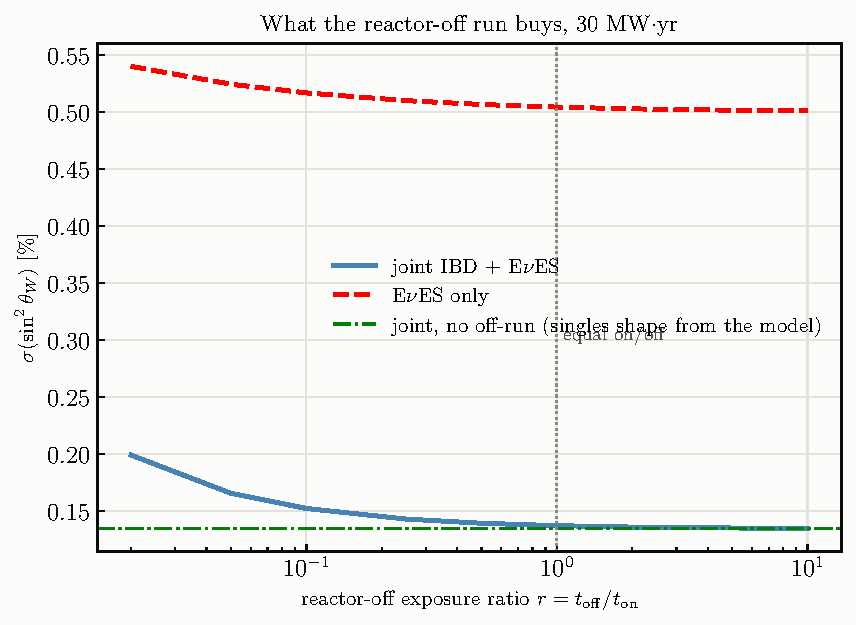
\includegraphics[width=\textwidth]{nb5_onoff}
\caption{$\sigma(\sw)$ against the reactor-off exposure ratio at $30\,\MWyr$.  Equal on/off
running ($r=1$) is within $2\%$ of the $r\to\infty$ asymptote and is the optimum at fixed
calendar time, \cref{eq:ropt}; a $2\%$-length off-run costs $45\%$ on the joint fit.  The
horizontal line is the separate analysis in which there is no off-run at all and the
singles shape is taken from the model.}
\label{fig:onoff}
\end{figure}

\begin{table}[t]\centering
\begin{tabular}{lccc}\toprule
singles rate assumed & rate [day$^{-1}$] & \eves{}-only & joint\\\midrule
none & $0$ & $0.474$ & $0.120$\\
$0.1\times$ nominal & $1.2\times10^4$ & $0.492$ & $0.130$\\
nominal (as modelled) & $1.2\times10^5$ & $0.504$ & $0.137$\\
$3\times$ nominal & $3.7\times10^5$ & $0.510$ & $0.144$\\
$10\times$ nominal & $1.2\times10^6$ & $0.520$ & $0.159$\\
$30\times$ nominal & $3.7\times10^6$ & $0.535$ & $0.193$\\
\bottomrule\end{tabular}
\caption{Robustness of $10^2\,\sigma(\sw)$ at $30\,\MWyr$ to the assumed singles level,
with equal reactor-on and reactor-off exposure.  A background $30\times$ larger than
modelled costs $41\%$; this is the payoff of measuring it rather than predicting it.}
\label{tab:onoff}
\end{table}

Two more things follow.  The answer is remarkably insensitive to the singles level
(\cref{tab:onoff}): $10\times$ the background costs $16\%$ and $30\times$ costs $41\%$.
And the fiducial radius barely matters: $\sigma(\sw)$ moves only from $0.134$ to $0.139$
between $R=15.5$ and $17.0$~m while the singles rate inside the cut moves by a factor of
six, because the reactor-off subtraction, not the cut, is doing the work.  I therefore
keep the $R=16.5$~m of the rest of this report rather than optimising a cut against
provisional rates.

\subsection{Neutrino interactions on $^{13}$C}
\label{sec:c13}
Natural carbon is $1.1\%$ $^{13}$C by atom, so the scintillator holds $\sim210$~t of it,
$9.7\times10^{30}$ nuclei, the target JUNO uses for its model-independent $^8$B measurement
\cite{Gavrikov:2025rlg}.  Both channels land in the single-hit window, and they behave very
differently here.

\paragraph{The neutral current is purely isovector axial.}
At the quark level the neutral current is
\begin{equation}
\mathcal{L}_{\rm NC}=-\frac{G_F}{\sqrt2}\,
\big[\bar\nu\gamma^\mu(1-\gamma_5)\nu\big]
\sum_q\bar q\gamma_\mu\big(g_V^q-g_A^q\gamma_5\big)q,
\label{eq:lnc}
\end{equation}
with $g_V^u=\tfrac12-\tfrac43 s_W^2$, $g_A^u=+\tfrac12$, $g_V^d=-\tfrac12+\tfrac23 s_W^2$
and $g_A^d=-\tfrac12$, $s_W^2\equiv\sw$.  Rearranged into isospin components this is the
familiar statement
\begin{equation}
J_\mu^{Z}=J_\mu^{3}-2s_W^2\,J_\mu^{\rm em},
\qquad J_\mu^{3}=V_\mu^{3}-A_\mu^{3},
\label{eq:jz}
\end{equation}
and because the electromagnetic current is purely vector, \emph{the entire axial part of the
neutral current is $-A_\mu^{3}$, the third isospin component of the axial current, carrying
coefficient exactly unity and no $s_W^2$ whatsoever}.  Only the vector part is mixed and
$s_W^2$-suppressed.  At the nucleon level, in the non-relativistic limit, the space
components of $A^3_\mu$ reduce to
\begin{equation}
A^{3}_{k}\;\longrightarrow\;\frac{g_A}{2}\sum_i\sigma_{k,i}\,\tau^3_i
\;+\;\frac{\Delta s}{2}\sum_i\sigma_{k,i},
\label{eq:a3}
\end{equation}
an isovector spin operator with coefficient $g_A=1.2754$ and an isoscalar one carried by
the strange-quark spin, $\Delta s\approx-0.08$, an order of magnitude smaller.

Now the transition does the rest of the work.  The $^{13}$C ground state is $J^\pi=1/2^-$
and the excited level is $3/2^-$: $\Delta J=1$ with no parity change.  The leading
(allowed) operator of the \emph{vector} current is the Fermi charge operator
$\sum_i\tau^3_i$, which is $\Delta J=0$ and therefore cannot connect the two states at all;
the vector current enters only through weak magnetism, $\propto\mu_V\,\bm\sigma\times\bm q/2M_N$,
suppressed by $q/2M_N\sim10^{-3}$ at these energies.  The leading operator of the
\emph{axial} current is precisely the $\Delta J=1$ spin operator of \cref{eq:a3}.  So the
line strength is
\begin{equation}
\sigma_{\rm NC}(E_\nu)=\frac{G_F^2}{\pi}\,(E_\nu-E_x)^2\,\frac{g_A^2}{4}\,B({\rm GT}^0)
\Big[1+\mathcal{O}\big(q/M_N,\ \Delta s/g_A\big)\Big],
\qquad
B({\rm GT}^0)\equiv\frac{\big|\langle f\|\sum_i\sigma_i\tau^3_i\|i\rangle\big|^2}{2J_i+1},
\label{eq:signc}
\end{equation}
with $E_x=3.685$~MeV and the $(E_\nu-E_x)^2$ from the phase space of the outgoing massless
neutrino.  The $1/4$ is the $\tau^3/2$ normalisation of the isospin current.

Two consequences are worth stating plainly.  First, \emph{the line carries no leading
dependence on $\sw$ at all}: it measures $g_A^2 B({\rm GT}^0)$, the isovector axial
strength.  It is therefore not a second weak-mixing-angle measurement but a genuinely
different observable, sensitive to the hadronic axial current where \eves{} is sensitive to
the electron couplings, and to any new physics that touches quark neutral currents without
touching electrons.  Second, the same isovector spin operator governs the $M1$ strength of
the $3.685$~MeV level, so $B({\rm GT}^0)$ is constrained by nuclear data rather than being a
free parameter.

\paragraph{Why the isoscalar axial current is so much harder.}
It is worth spelling out what the neutral current does \emph{not} contain.  In
\cref{eq:lnc} the axial couplings satisfy $g_A^u=-g_A^d=+\tfrac12$, so the up and down
isoscalar axial contributions cancel identically and, within $u,d,s$,
\begin{equation}
A_\mu^{Z}=\tfrac12\big(\bar u\gamma_\mu\gamma_5u-\bar d\gamma_\mu\gamma_5 d\big)
-\tfrac12\,\bar s\gamma_\mu\gamma_5 s
\;\longrightarrow\;
\tfrac12 g_A\,\tau^3\;-\;\tfrac12\Delta s ,
\label{eq:isoscalar}
\end{equation}
so the entire isoscalar axial piece is carried by the strange-quark spin.  That makes it a
clean probe of $\Delta s\approx-0.08$, and hence of the proton spin decomposition, but it
also makes it small: $\Delta s/g_A\approx1/16$.

There are only two ways to get at it, and neither survives reactor energies.  One can
isolate it with a transition that the isovector operator cannot drive at all, namely
$T=0\to T=0$ with $\Delta J=1$ in a self-conjugate nucleus, since $\tau^3$ is an isovector
and cannot connect two $T=0$ states.  The textbook case is the $12.71$~MeV $1^+,T=0$ level
of $^{12}$C, measured against the isovector $15.11$~MeV $1^+,T=1$ level.  But the rate then
costs $(\Delta s/g_A)^2\approx4\times10^{-3}$, and $12.71$~MeV sits above the reactor
endpoint of $\sim10$~MeV in any case; the low-lying $T=0\to T=0$ alternatives
($^{6}$Li at $4.31$~MeV, $^{10}$B at $3.59$~MeV) are either particle-unbound or present in
far too small a quantity.  The alternative is to let the isoscalar amplitude
\emph{interfere} with the isovector one, which buys linear rather than quadratic
sensitivity but requires both to reach the same final state, i.e.\ a free nucleon.  That is
elastic $\nu p\to\nu p$, the BNL~E734 measurement.  At reactor energies the proton recoil is
$T_p=2E_\nu^2/M_p\lesssim0.14$~MeV, quenched to $\sim10$~keV of visible energy in
scintillator, far below any threshold.  The isoscalar axial current is therefore out of
reach here, and the $^{13}$C line remains an isovector measurement.

\paragraph{The charged current is neutrino-only, and empirically normalised.}
For $\nu_e+{}^{13}\mathrm{C}\to e^-+{}^{13}\mathrm{N}$(g.s.) the allowed cross section is
\begin{equation}
\sigma_{\rm CC}(E_\nu)=\frac{G_F^2\cos^2\theta_C}{\pi}\,p_eE_e\,F(Z{=}7,E_e)
\big[B(\mathrm{F})+g_A^2B(\mathrm{GT})\big],\qquad E_e=E_\nu-Q+m_e,
\label{eq:sigcc}
\end{equation}
with $E_e$ the total electron energy and $Q=2.22$~MeV the threshold, which is just the
$^{13}$N--$^{13}$C atomic mass difference, the electron created and the one shed by the
change in $Z$ cancelling.  Here $^{13}$N(g.s.) is the isobaric analog of $^{13}$C(g.s.) (a $T=1/2$
doublet with $T_3=\pm1/2$), so the Fermi matrix element is unquenched, $B(\mathrm{F})=1$,
and the combination $B(\mathrm{F})+g_A^2B(\mathrm{GT})$ is fixed directly by the measured
$ft$ value of the mirror $^{13}\mathrm{N}\to{}^{13}\mathrm{C}\,e^+\nu_e$ decay.  The CC
cross section is thus known without a nuclear model.

Crucially this channel needs a \emph{neutrino}.  The antineutrino partner is
$\bar\nu_e+{}^{13}\mathrm{C}\to e^++{}^{13}\mathrm{B}$, and its threshold follows from the
nuclear masses: the atomic mass excesses give
$\Delta M_{\rm at}=16.562-3.125=13.437$~MeV, converting to nuclear masses adds one electron
mass since $Z$ drops from $6$ to $5$, and creating the positron costs another, so
\begin{equation}
E_{\rm th}=\big[M_{\rm nuc}({}^{13}\mathrm{B})-M_{\rm nuc}({}^{13}\mathrm{C})\big]+m_e
=\Delta M_{\rm at}+2m_e=14.46\ \mathrm{MeV}.
\label{eq:13Bthreshold}
\end{equation}
That is half again the reactor endpoint of $\sim10$~MeV, so the reactor contributes nothing
to it and the CC channel is a purely solar background, tagged besides by the $863$~s
$^{13}$N $\beta^+$ coincidence.
The neutral current, by contrast, is flavour blind and identical for neutrinos and
antineutrinos, so \emph{the reactor antineutrinos excite it}.  The level lies below the
$4.946$~MeV neutron separation energy, so it is particle bound and de-excites by a single
$3.685$~MeV $\gamma$: a monoenergetic line, $73$~keV wide at JUNO's resolution, landing a
full MeV above the $2.615$~MeV wall in the cleanest part of the window.

\paragraph{Rates.}
I take the energy dependence from \cref{eq:signc,eq:sigcc} and fix the two overall scales by
JUNO's own $^8$B yields, $3032$ NC and $3929$ CC events in ten years, rather than by
evaluating $B({\rm GT}^0)$ from a shell model.  Carrying that law from the $^8$B weighting
($3.7$--$15$~MeV) down to the reactor's ($3.7$--$9$~MeV) is a modest extrapolation, so the
reactor rate should be read as good to a factor of order unity.  It gives $4.1$ events per
day at $10\,\mathrm{MW}$ and $50$~m, five times the solar NC rate, and as a background to
\eves{} it is negligible: including all of the $^{13}$C moves $\sigma(\sw)$ by one digit in
the fifth place.  Note that the $^{13}$C count cancels exactly between the anchoring and
the prediction, so the rate does not depend on it.

As a measurement in its own right it is more interesting.  Treating the line normalisation
as the parameter of interest, with its cross-section prior dropped and every other
systematic standing, the reactor-driven line reaches $\mathbf{12\sigma}$ at $30\,\MWyr$
($4.5\times10^3$ events; $7.0\sigma$ at $10\,\MWyr$, $21\sigma$ at $100\,\MWyr$).  It is
the one place in the window where a sharp feature sits on a smooth continuum, so it is
limited by statistics rather than by any shape systematic.

\subsection{Neutrino interactions on deuterium}
\label{sec:deuterium}
Natural hydrogen carries $156$~ppm of deuterium, so JUNO's $1.44\times10^{33}$ free protons
come with $2.2\times10^{29}$ deuterons, about $750$~kg of D, $2.3\%$ of the $^{13}$C count.
Deuterium is the target one would most like to have: the neutral-current breakup
$\nu+d\to\nu+n+p$ is a pure Gamow-Teller transition on the simplest of all nuclei, with a
matrix element known from pionless effective field theory to about $1\%$ rather than from a
shell model, and it is how SNO measured the total solar flux.  Two channels are open, and their thresholds are worth assembling piece by piece because the
gap between them is what decides everything that follows.  Both must first pay the deuteron
binding energy,
\begin{equation}
B_d=m_p+m_n-M_d=938.272+939.565-1875.613=2.224\ \mathrm{MeV}.
\label{eq:bd}
\end{equation}
The neutral current pays nothing else, since the outgoing neutrino is massless and the
final state is just an unbound $np$ pair.  The charged current must in addition turn a
proton into a neutron and materialise a positron,
\begin{align}
\bar\nu_e+d&\to \bar\nu_e+n+p,
&E_{\rm th}&=B_d=2.224\ \mathrm{MeV},
\label{eq:ncd}\\
\bar\nu_e+d&\to e^++n+n,
&E_{\rm th}&=B_d+(m_n-m_p)+m_e=2.224+1.293+0.511=4.028\ \mathrm{MeV},
\label{eq:ccd}
\end{align}
the second of which is just $2m_n+m_e-M_d$ written in a more transparent way.  Folding
these against the reactor spectrum, the neutral current samples $71.4\%$ of the flux and
the charged current only $14.5\%$ of it, a factor of five that the cross sections more than
undo: the charged current is the larger of the two per neutrino, by a factor $\sim2.5$ at
these energies, as SNO's two channels also show.

As for $^{13}$C the energy dependence is derived and the two overall scales are external.
Both channels are allowed transitions, so a lepton of energy $E_\ell$ recoils against a
two-body continuum of relative energy $\epsilon$ whose density of states goes as
$\sqrt\epsilon$,
\begin{equation}
\sigma_{\rm NC}\propto\int_0^{Q}(Q-\epsilon)^2\sqrt\epsilon\,d\epsilon\propto Q^{7/2},
\qquad
\sigma_{\rm CC}\propto\int_0^{Q'}p_eE_e\sqrt\epsilon\,d\epsilon,
\label{eq:dshapes}
\end{equation}
with $Q=E_\nu-B_d$ and $E_e=Q'-\epsilon+m_e$, $Q'=E_\nu-4.028\,\mathrm{MeV}$.  This omits
the $^1S_0$ final-state interaction, which enhances small $\epsilon$ in \emph{both}
channels and so largely cancels between them.  The scales are the per-fission cross
sections at $^{235}$U-dominated reactors, well matched to the HALEU core,
$\sigma_{\rm CC}=1.06\times10^{-44}$ and $\sigma_{\rm NC}=5.6\times10^{-45}\,
\mathrm{cm^2/fission}$, on which theory and the reactor measurements agree to about
$10\%$; every number below inherits that $10\%$ and nothing worse.  The raw rates at
$10\,\mathrm{MW}$ and $50$~m are then $0.157$ (CC) and $0.084$ (NC) events per day.

The two channels then part company completely, and it is the signature rather than the rate
that decides.  The charged current gives a prompt positron followed by \emph{two} neutron
captures, a triple coincidence, and the two neutrons share a vertex.  The only serious
accidental is an ordinary IBD event picking up a second neutron from another IBD, and
requiring the second capture within $1$~m and $1$~ms of the first reduces that to
$9\times10^{-3}$ per day against a signal of $0.157$ per day.  That is $172$ events
per $30\,\MWyr$ at $13\sigma$, and the significance is signal-statistics limited
rather than background limited.  Note that both signal and accidental scale with reactor
power, so the signal-to-background is a property of the vertex cut and not of the exposure.
The background that would need real work is cosmogenic fast neutrons, which genuinely
produce multi-neutron events.

The neutral current, by contrast, produces a lone $2.22$~MeV neutron-capture $\gamma$ with
no prompt at all, since the proton recoil is sub-MeV and heavily quenched.  Against
$5\times10^3$ singles per day in the surrounding $0.45$~MeV, and even with equal reactor-off
subtraction, this reaches $0.02\sigma$.  It is inaccessible.  The channel one wants is
precisely the one the abundance denies: a deuterated target would be needed, and doping the
scintillator to $1\%$ D would give $10$ CC and $5$ NC events per day, while a dedicated
one-tonne D$_2$O cell at $10$~m would give $1.1$ and $0.6$.  Neither is a modification to
JUNO; both are separate experiments.  What the parked reactor does deliver for free is a
respectable $\bar\nu_e d$ charged-current measurement riding on the same data as everything
else.

\subsection{Systematics}
The \eves{}-only fit carries the following modes: a $2\%$ normalisation
(power$\times$target$\times$efficiency); the \eves{} cross-section normalisation at
$0.2\%$ (the $O(\alpha)$ radiative corrections, the only theory error left once the
couplings are the parameters of interest); the 25-mode measured $^{235}$U shape covariance
\cite{DayaBay:2021dqj}; $^{238}$U at $\pm15\%$; the IBD-singles normalisation at
$\pm10\%$; solar at $\pm3\%$; energy scale, bias and resolution at $0.5/0.5/5\%$,
coherent between the electron and positron responses, plus a $0.2\%$ scale mode on the
electron response alone; and the fuel-evolution (Pu-ingrowth) mode at $\pm30\%$.  The detector singles carry no normalisation prior at all: under
\cref{eq:onoff} their level and shape are measured, and what remains is a $1\%$ coherent
\emph{stability} residual between the on and off periods (radon drift, muon-rate
variation).  That residual is a complete null: even a $10\%$ residual leaves
$\sigma(\sw)$ unchanged at five digits, because the steeply-falling singles shape is
nearly orthogonal to the coupling-induced distortion of the recoil spectrum.

The joint fit stacks the IBD anchor spectrum ($1.0$--$9.0$~MeV in 50~keV bins) with the
\eves{} spectrum, \emph{frees the flux normalisation} (a loose 10\% prior) and lets the IBD
channel measure it.  The transfer to \eves{} is then limited by four terms: the channel
ratio $N_e/N_p\times\varepsilon$ ($0.5\%$), the IBD cross-section normalisation ($0.2\%$,
from $\tau_n$ and radiative corrections \cite{Vogel:1999zy,Strumia:2003zx}) with a
zero-mean linear tilt on top ($0.1\%$), the \eves{} cross-section normalisation ($0.2\%$),
and the residual $e^-$/$e^+$ energy-scale difference ($0.2\%$).  The last of these deserves
a word.  Freeing the flux normalisation is what lets the anchor pin the energy response,
and it does so only to the extent that the electron and positron scales move together;
they are calibrated with different sources, since an electron deposits one continuous
track and a positron its kinetic energy plus two $511$~keV quanta.  The decorrelated
residual is therefore carried, and it costs $8\%$ of the final number.  Under the anchor the standard JUNO
backgrounds (far reactors, geoneutrinos, $^9$Li/$^8$He, world reactors, $^{214}$Bi--Po and
``other'', about $45$ per day against $5.8\times10^4$ per day) enter at their release priors
\cite{JUNO:2025gmd}, and the shared $^{235}$U shape modes act on both channels
coherently, so the anchor constrains them in situ.

\subsection{Results}
\label{sec:results}
\Cref{tab:sw2} decomposes $\sigma(\sw)$ at $30\,\MWyr$, and \cref{fig:sw2exp} shows the
exposure dependence.

\begin{table}[t]\centering
\begin{tabular}{lc}\toprule
\eves{}-only variant, $30\,\MWyr$ & $10^2\,\sigma(\sw)$\\\midrule
all systematics & $0.504$\\
no flux-shape covariance & $0.352$\\
no detector singles & $0.474$\\
no solar/JUNO backgrounds & $0.503$\\
no energy scale/bias/res.\ pulls & $0.490$\\
no fuel-evolution mode & $0.502$\\
signal statistics only & $0.011$\\
\quad with the measured backgrounds & $0.030$\\\midrule
joint IBD+\eves{}, defaults & $0.137$\\
\quad IBD xsec $0.5\%$ (Strumia--Vissani) & $0.163$\\
\quad channel ratio $0.2\%$ & $0.103$\\
\quad $e^-/e^+$ relative scale $0.1\%$ & $0.130$\\
\quad all four transfer terms at best & $0.080$\\
\quad no $^{235}$U shape covariance & $0.133$\\
\quad no detector singles & $0.120$\\
\quad $2\%$-length reactor-off run ($r=0.02$) & $0.199$\\
\quad no reactor-off run, singles shape modelled & $0.135$\\
\bottomrule\end{tabular}
\caption{Precision on $\sw$ for $30\,\MWyr$ near-reactor exposure ($\approx3.3$ calendar
years with about $90\%$ uptime).  Entries are $10^2$ times the \emph{absolute} error, so
$0.137$ means $\sigma(\sw)=1.4\times10^{-3}$, or $0.6\%$ of $\sw$ itself.  ``All four
transfer terms at best'' is IBD xsec $0.1\%$, channel ratio $0.2\%$, \eves{} xsec $0.1\%$
and relative scale $0.1\%$.}
\label{tab:sw2}
\end{table}

\begin{figure}[t]\centering
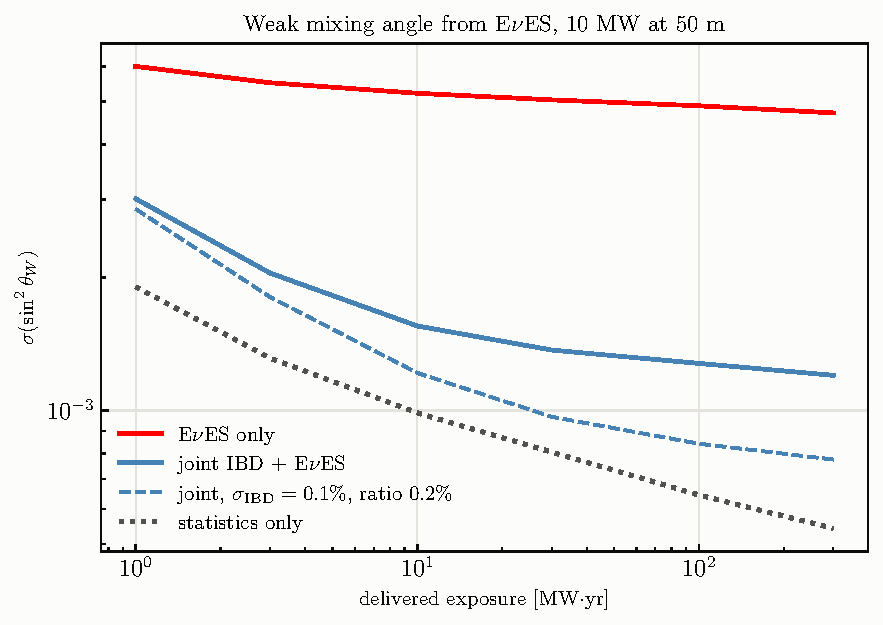
\includegraphics[width=\textwidth]{nb5_sigma_sw2_vs_exposure}
\caption{$\sigma(\sw)$ versus delivered exposure.  The \eves{}-only fit saturates on the
measured flux-shape covariance; the IBD-anchored fit converts statistics into precision
until it reaches its own floor, the transfer budget.}
\label{fig:sw2exp}
\end{figure}

Three structural conclusions come out of this.  First, \emph{the \eves{}-only measurement is
limited by the flux shape}: the recoil shape breaks the normalisation degeneracy far better
than the naive rate argument ($|d\ln R/d\sw|=4.75$) suggests, but the $2$--$4\%$
correlated bin uncertainties of the measured $^{235}$U spectrum imitate the coupling-induced
shape change and saturate the precision at $\sigma(\sw)\approx5\times10^{-3}$ regardless of
exposure.  Second, \emph{the joint fit removes that wall}: with the normalisation freed and
measured by the anchor, the $^{235}$U shape covariance and the coherent energy pulls become
near-nulls (the $7\times10^7$-event anchor pins both), and what remains is the transfer
budget, then the detector singles, then the fuel-evolution mode and the solar/JUNO
backgrounds.  The result, $\sigma(\sw)=1.4\times10^{-3}$ at $30\,\MWyr$ and
$8.0\times10^{-4}$ at the plausible best of the transfer inputs, is a
$\sim0.6\%$-of-itself low-energy weak mixing angle, competitive with the best existing
determinations \cite{Erler:2004in}.

Third, and this is worth stating plainly because it says what the measurement actually
requires: \emph{the joint number is a rate ratio and almost nothing else}.  Adding the four
transfer priors in quadrature and dividing by $|d\ln R/d\sw|$ gives
$\sqrt{0.5^2+0.2^2+0.2^2+0.2^2}\%/4.75=1.3\times10^{-3}$, which is $92\%$ of the full
answer; the spectral information contributes the rest.  The exposure dependence of
\cref{fig:sw2exp} flattens for the same reason.  So the claim of this section is
conditional in a specific and testable way: \emph{if} $N_e/N_p\times\varepsilon$ can be
established to $0.5\%$ and $\sigma_{\rm IBD}$ to $0.2\%$, the parked reactor delivers
$\sigma(\sw)=1.4\times10^{-3}$.  Establishing the first of those is a scintillator-assay
and efficiency question, not a neutrino one, and it is where the effort belongs.

\Cref{fig:gvga} shows the same anchoring in the $(g_V,g_A)$ plane: $\sigma(g_V)=0.0038$ and
$\sigma(g_A)=0.0072$ at $30\,\MWyr$, with principal semi-axes $0.0026\times0.0077$.  The
singles cost $g_A$ far more than $g_V$, as they must: $g_A$ is fixed by the low-recoil
shape, which is exactly where they live.

\Cref{fig:gvga_land} places this in the existing landscape.  Electron-flavour experiments
see the CC amplitude too, so their cross sections depend on $(g_V+1,\,g_A+1)$ and constrain
\emph{bands} along the resulting degeneracies rather than ellipses: $\nu_ee$ (LSND
\cite{LSND:2001akn}, LAMPF \cite{Allen:1992qe}) bounds
$(g_V+g_A+2)^2+(g_V-g_A)^2/3=2.34\pm0.35$, and $\bar\nu_ee$ (TEXONO \cite{TEXONO:2009knm})
bounds $(g_V-g_A)^2+(g_V+g_A+2)^2/3$ through $\xi=\sigma/\sigma_{\rm SM}=1.08\pm0.26$.
Muon-flavour scattering (CHARM~II \cite{CHARM-II:1994dzw}: $g_V=-0.035\pm0.017$,
$g_A=-0.503\pm0.017$; BNL~E734 \cite{Ahrens:1990fp}: $-0.107\pm0.045$, $-0.514\pm0.036$)
is pure NC and gives ellipses; the PDG world average, $g_V=-0.040\pm0.015$ and
$g_A=-0.507\pm0.014$ \cite{ParticleDataGroup:2024cfk}, is dominated by CHARM~II and
assumes flavour universality.  Neutrino trident production (CCFR \cite{CCFR:1991lpl},
$\sigma/\sigma_{\rm SM}=0.82\pm0.28$; CHARM~II \cite{CHARM-II:1990dvf}, $1.58\pm0.57$)
constrains the $\nu_\mu$--\emph{muon} couplings \cite{Altmannshofer:2014pba} rather than
$\nu$--$e$, so I do not draw it.  Reactor $\bar\nu_ee$ data combined give
$\sw=0.252\pm0.030$ \cite{Canas:2016vxp}.  Our measurement is $\bar\nu_e$: it lands on
TEXONO's band and shrinks it by nearly two orders of magnitude, and its joint 30~MW\,yr
ellipse sits inside the CHARM~II and world-average circles, $4.5\times$ tighter in $g_V$
and $2.4\times$ in $g_A$ (and $2.2$--$6.7\times$ along its principal axes), from a
different flavour.  All contours are
centred on the PDG world-average point.

\begin{figure}[t]\centering
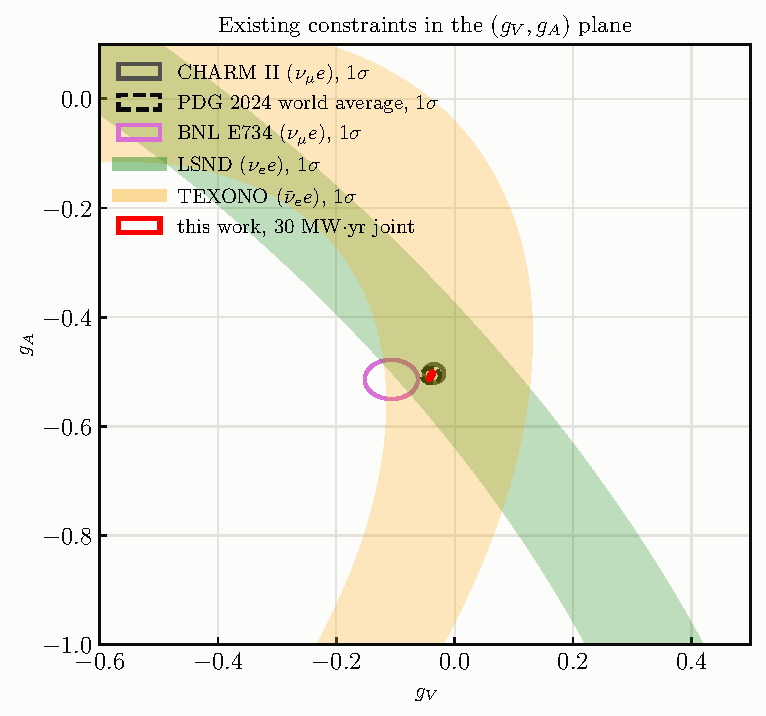
\includegraphics[width=\textwidth]{nb5_gv_ga_landscape}
\caption{Existing $1\sigma$ constraints in the $(g_V,g_A)$ plane: the $\nu_ee$ (LSND) and
$\bar\nu_ee$ (TEXONO) bands, the $\nu_\mu e$ ellipses (CHARM~II, BNL~E734) and the PDG
world average, with this work's 30~MW\,yr joint region at the PDG point.}
\label{fig:gvga_land}
\end{figure}
\begin{figure}[t]\centering
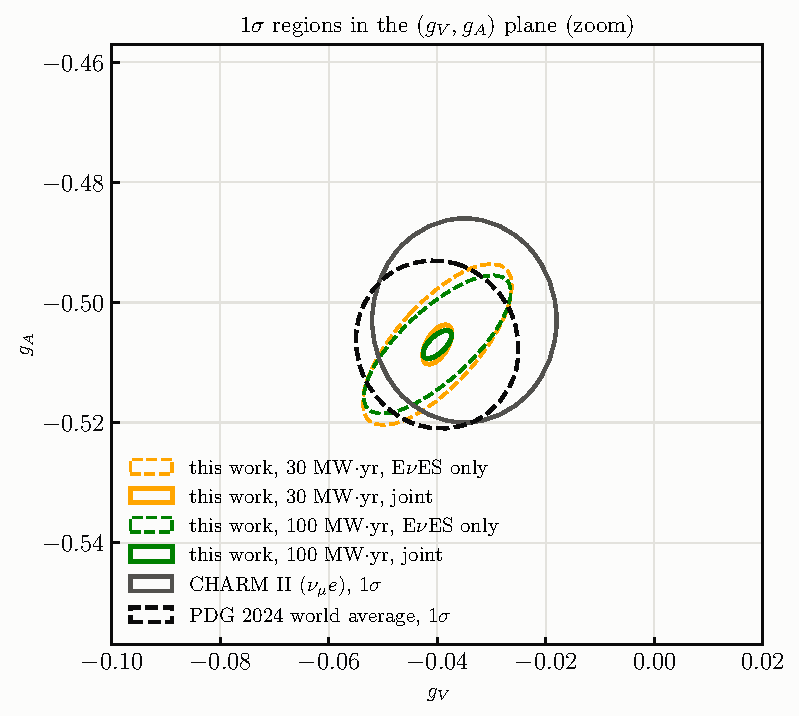
\includegraphics[width=\textwidth]{nb5_gv_ga_ellipses}
\caption{Zoom on the PDG point: $1\sigma$ Fisher regions of this work, \eves{}-only
(dashed) and IBD-anchored (solid), against the CHARM~II and PDG world-average ellipses.}
\label{fig:gvga}
\end{figure}

%======================================================================
\section{Sterile-neutrino wiggles across the finite detector (notebook 6)}
\label{sec:sterile}

\subsection{The idea}
Start from the geometry, because it is the whole reason this works.  Put a point source at
distance $D$ from the centre of a fiducial sphere of radius $R$ and ask how much target
sits at baseline $L$.  The locus of points at fixed $L$ from the source is a sphere, and the
part of it inside the detector is a spherical cap.  With $\alpha$ the polar angle measured
from the source-to-centre axis, the cap edge is where the two spheres intersect, given by
the cosine rule as
\begin{equation}
\cos\alpha_{\max}(L)=\frac{L^{2}+D^{2}-R^{2}}{2LD},
\label{eq:capangle}
\end{equation}
so the cap area is $2\pi L^{2}\big[1-\cos\alpha_{\max}\big]$ and the target volume between
$L$ and $L+dL$ is
\begin{equation}
A(L)=2\pi L^{2}\left[1-\frac{L^{2}+D^{2}-R^{2}}{2LD}\right],
\qquad |D-R|\le L\le D+R .
\label{eq:AL}
\end{equation}
The event density then carries the usual inverse-square dilution,
\begin{equation}
\frac{dN}{dL}\propto\frac{A(L)}{L^{2}}
=2\pi\left[1-\frac{L^{2}+D^{2}-R^{2}}{2LD}\right],
\label{eq:dNdL}
\end{equation}
which is exact, contains no free parameter, and is worth pausing on: the $L^{2}$ of the cap
area cancels the $1/L^{2}$ of the flux, leaving a distribution fixed entirely by $D$ and
$R$.  Nothing about the reactor enters it.  At $D=50$~m and $R=16.5$~m the baseline spans
$33$ to $67$~m, a factor of two.  For $\dm{41}\sim0.1$--$10\,\mathrm{eV^2}$ the oscillation
length at reactor energies is metres to tens of metres, so the disappearance pattern
\emph{wiggles across the detector} (\cref{fig:wiggle_map,fig:wiggle_slices}).  Binning
events in reconstructed vertex baseline $L$ makes JUNO a many-baseline experiment in one
fill, and no flux or cross-section systematic can follow: the geometry is exact and the
source spectrum carries no $L$-dependence.

\begin{figure}[t]\centering
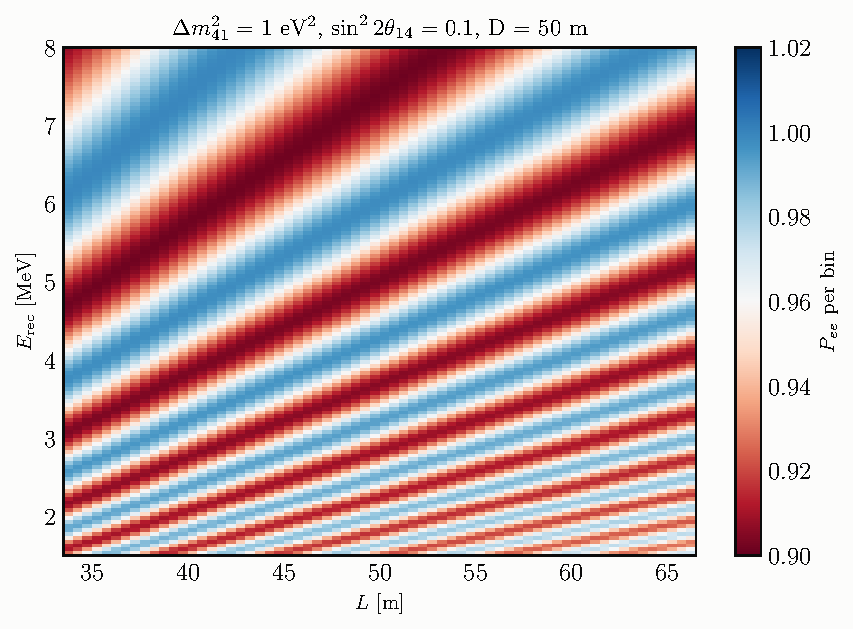
\includegraphics[width=\textwidth]{nb6_wiggle_map}
\caption{Survival probability per $(L,E_{\rm rec})$ bin for $\dm{41}=1\,\mathrm{eV^2}$,
$\st{14}=0.1$, $D=50$~m.}
\label{fig:wiggle_map}
\end{figure}
\begin{figure}[t]\centering
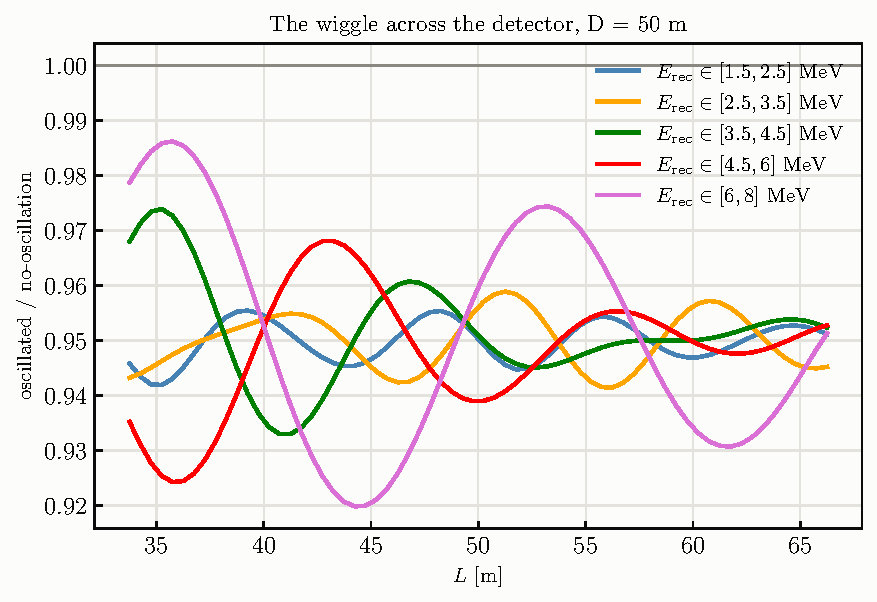
\includegraphics[width=\textwidth]{nb6_wiggle_slices}
\caption{The same benchmark: oscillated/unoscillated ratio versus $L$ in five energy
windows across the spectrum.  The wavelength scales as $E$ ($\sim5$~m at 2~MeV, $\sim20$~m
at 7~MeV), so different energies sample the same $L$ range with different phase advance;
this $(L,E)$ pattern is what no source systematic can mimic.}
\label{fig:wiggle_slices}
\end{figure}

\subsection{Oscillation, smearing, statistics}
I use the full 3+1 vacuum survival probability,
\begin{equation}
P_{ee}=1-(1-s_{14})^2\,(1-P^{3\nu}_{ee})-4s_{14}(1-s_{14})\sum_{i=1}^{3}|U_{ei}|^2_{3\nu}
\sin^2\Delta_{i4},\qquad s_{14}=\sin^2\theta_{14},
\end{equation}
with the exact three-flavour $P^{3\nu}_{ee}$ in the $\dmee$ parameterisation
\cite{Minakata:2006gq} and $\Delta_{i4}=1.267\,(m_4^2-m_i^2)L/E$
($\dm{31}=\dmee+s_{12}^2\dm{21}$).  I validated it against a brute-force PMNS-amplitude
computation to $8.5\times10^{-6}$.  Expanding the $(1-s_{14})^2$ prefactor,
$1-(1-s_{14})^2=\tfrac12\st{14}+O(\st{14}^2)$, so the prediction is exactly affine in
$\st{14}$ to first order with the template
\begin{equation}
W=\sum_{i}|U_{ei}|^2_{3\nu}\sin^2\Delta_{i4}-\tfrac12\big(1-P^{3\nu}_{ee}\big),
\label{eq:wtemplate}
\end{equation}
the second term being the piece of the ordinary $\theta_{13}$ disappearance that the
sterile mixing switches off.  It is $6\times10^{-4}$ of the first at 50~m and $\sim3\%$ at
$1.4$~km, and it carries no $L$-wiggle.  At 50~m the whole expression reduces to
$1-\st{14}\sin^2\Delta_{41}$,
while at $1.4$~km, where $\Delta_{31}\approx1$~rad, the three sterile phases separate and
the null hypothesis is the $\theta_{13}$-oscillated spectrum.  IBD (CC) and \eves{}
(CC+NC) deplete identically, since an oscillated $\bar\nu_e$ is sterile; the
$\bar\nu_{\mu,\tau}$ that the standard oscillation produces still scatters by NC and is
carried with its own cross section, so the \eves{} null is exact at every standoff.

Two effects smear the true baseline at fixed reconstructed vertex, and both damp the
wiggle in the same way, so it is worth deriving the damping once.  Write the oscillating
factor as $\sin^{2}kL$ with $k=1.267\,\dm{}/E$ in units of $\mathrm{eV^{2}}$, MeV and
metres, and suppose the true $L$ is Gaussian-distributed about the reconstructed value with
variance $\sigma_L^{2}$.  Using $\sin^{2}kL=\tfrac12[1-\cos2kL]$ and the standard Gaussian
average of a cosine, $\langle\cos2kL\rangle=\cos(2k\bar L)\,e^{-2k^{2}\sigma_L^{2}}$,
\begin{equation}
\big\langle\sin^{2}kL\big\rangle
=\tfrac12\Big[1-\cos(2k\bar L)\,e^{-2k^{2}\sigma_L^{2}}\Big].
\label{eq:damping}
\end{equation}
The mean survives untouched and only the oscillating part is attenuated, by
$e^{-2k^{2}\sigma_L^{2}}$.  Counts are therefore conserved by the smearing, which is why
the null spectra are unaffected by it and only the signal template is damped.

The two contributions to $\sigma_L^{2}$ add in quadrature.  A finite core of radius $a$,
uniformly emitting, has a line-of-sight coordinate distributed as the projection of a
uniform ball, whose variance is
$\langle z^{2}\rangle=\tfrac{1}{V}\!\int z^{2}\,d^{3}r=a^{2}/5$.  The vertex resolution
contributes $\sigma_1^{2}/E$ for a JUNO-like $\sigma_{\rm vtx}=\sigma_1/\sqrt{E}$.  Hence
\begin{equation}
\sigma_L^{2}=\frac{\sigma_1^{2}}{E}+\frac{a^{2}}{5},
\label{eq:sigmaL}
\end{equation}
and since the exponent goes as $k^{2}\propto(\dm{}/E)^{2}$, the damping switches on
quadratically in $\dm{}$.  This is what terminates the reach at high $\dm{}$, and
\cref{eq:sigmaL} shows immediately which term does it: the core radius enters with no
energy dependence, so once $a^{2}/5$ exceeds $\sigma_1^{2}/E$ the source, not the detector,
sets the wall.  Averaging over the finite width of an $L$ bin is done exactly with
sub-nodes rather than analytically.

The statistics then simplify remarkably.  The sterile term in $P_{ee}$ enters multiplied by
$\st{14}$ and nothing else, so the predicted spectrum is affine in that one parameter,
\begin{equation}
\bm\mu(\st{14})=\bm\mu_0-\st{14}\,\bm W(\dm{}),
\label{eq:affine}
\end{equation}
where $\bm\mu_0$ is the three-flavour null and $\bm W$ is a single wiggle template per
$\dm{}$, built once.  Putting \cref{eq:affine} into the Asimov quadratic form
\cref{eq:fisher} with $\bm\theta_0$ the null,
\begin{equation}
\Delta\chi^{2}(\dm{},\st{14})=\st{14}^{2}\;\bm W^{T}C^{-1}\bm W
\;\equiv\;\st{14}^{2}\,Q(\dm{}),
\label{eq:sterilechi2}
\end{equation}
so a single number $Q$ per $\dm{}$ carries the entire sensitivity and the exclusion curve
is closed-form,
\begin{equation}
\st{14}^{\rm excl}(\dm{})=\sqrt{\frac{\Delta\chi^{2}_{\rm crit}}{Q(\dm{})}},
\qquad \Delta\chi^{2}_{\rm crit}=5.99\ (95\%\ \mathrm{CL},\ 2\ \mathrm{dof}).
\label{eq:sterilelimit}
\end{equation}
No scan over $\st{14}$ is needed at all, which is what makes the four-standoff, many-mode
analysis of \cref{fig:landscape} tractable.

\subsection{Why the analysis is shape-only, and what that costs}
The Daya Bay $^{235}$U spectrum was \emph{measured} at $\sim500$~m: a sterile with
$\dm{41}\sim0.1$--$3\,\mathrm{eV^2}$ would have depleted it by $\approx\st{14}/2$ in
normalisation ($4.8$--$5.0\%$ at $\st{14}=0.1$, computed) and left a $\lesssim1\%$ energy
tilt.  Using its normalisation or shape as a prior would inject the very signal being
searched for.  The standard analysis therefore leaves the flux normalisation
\emph{completely free} and the reactor $E$-shape \emph{completely free} (one unconstrained
mode per $E$ and per $T$ bin, coherent across $L$; 263 modes in total).  Only the
$L$-direction wiggle structure at fixed $E$ can then carry sterile information, and it
carries essentially all of it: relative to a Daya-Bay-prior analysis the limits move by
less than $0.5\%$ across $0.03$--$3\,\mathrm{eV^2}$, and by $11\%$ only at the
$10\,\mathrm{eV^2}$ wall.  The Daya Bay spectrum serves only as a shape template for event
rates.  The remaining nuisances are the detector response non-uniformities across the volume, the
fuel evolution ($\pm30\%$, a null), and the IBD/\eves{} ratio ($0.5\%$).  The
non-uniformities are the systematics that live in the wiggle direction and both are
modelled as Gaussian-correlated fields over $L$ with a $1.5$~m correlation length, so that
finer binning cannot manufacture high-frequency freedom.  One is an \emph{efficiency}
field ($0.5\%$), which is energy independent and is therefore broken by the
$E$-dependence of the oscillation phase.  The other is a position-dependent \emph{energy
scale} ($0.2\%$) --- the light collection against radius --- which does distort the
spectrum in $E$ as a function of $L$, the same joint direction the signal lives in, and is
the more dangerous of the two.  It is still not the limiter: the field spans only
$\sim20$ correlated modes across a $33$~m span, which the fit projects out, so its cost
saturates and $0.2\%$ and $1\%$ give the same limit to three digits.  Together the two
fields cost under $1\%$ of the reach.  The backgrounds of \cref{sec:sm} (IBD singles, solar,
and the standard JUNO components distributed as volume in $L$) are included and shift the
limits by less than $0.1\%$: being smooth in both $L$ and $E$, they cannot make wiggles.

\subsection{Results}
\Cref{fig:landscape} shows the $95\%$~CL reach for $27\,\MWyr$ at each of five standoffs
against the existing landscape (DANSS \cite{DANSS:2018fnn}, PROSPECT
\cite{PROSPECT:2020sxr}, STEREO \cite{STEREO:2022nzk}, RENO+NEOS \cite{RENO:2020hva},
Gallium $2\sigma$ \cite{Barinov:2021asz,Berryman:2021yan}, KATRIN 2025
\cite{KATRIN:2025lph}, and the IsoDAR@Yemilab projection \cite{Alonso:2021jxx}).
\Cref{fig:lbin} isolates what the finite size buys, and \cref{fig:wall} the high-$\dm{}$
wall.

\begin{figure}[t]\centering
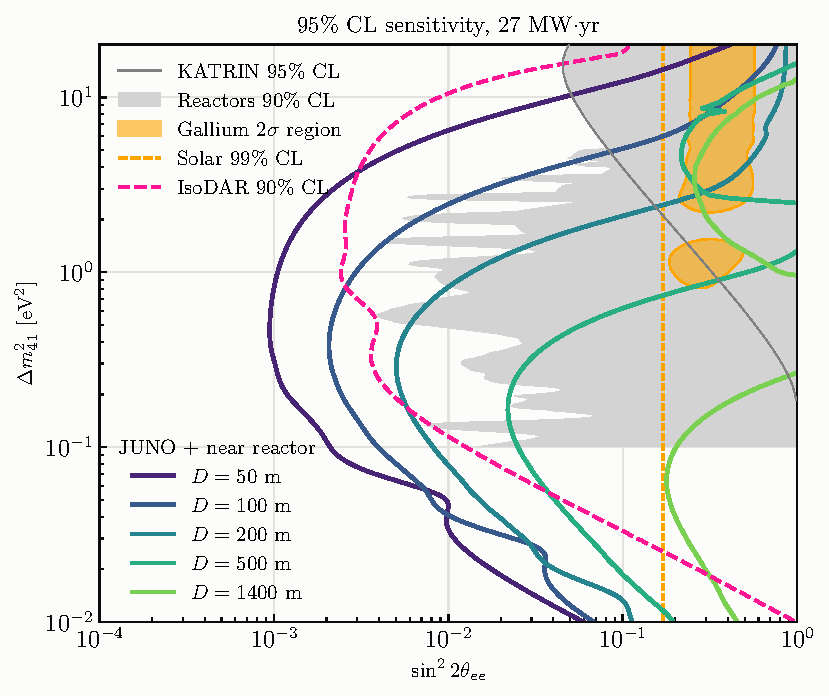
\includegraphics[width=\textwidth]{nb6_sensitivity_landscape}
\caption{$95\%$~CL sensitivity in the $\bar\nu_e$-disappearance plane for
$27\,\MWyr$ at $D=50$, $100$, $200$, $500$ and $1400$~m (each standoff separately), against
the reactor short-baseline exclusions (DANSS, PROSPECT, STEREO, RENO+NEOS; grey), KATRIN
2025, the Gallium $2\sigma$ region, the solar bound, and the IsoDAR@Yemilab projection.}
\label{fig:landscape}
\end{figure}
\begin{figure}[t]\centering
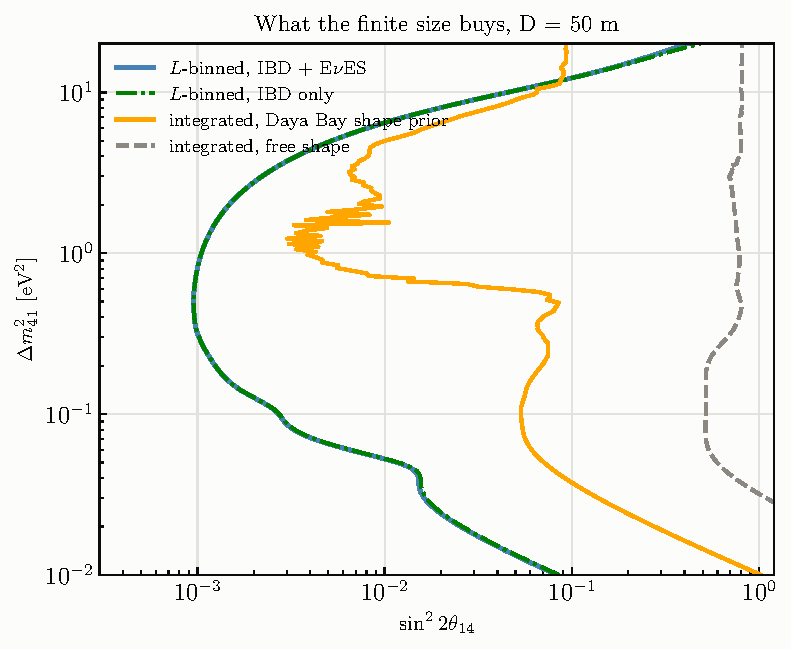
\includegraphics[width=\textwidth]{nb6_lbinned_vs_integrated}
\caption{The vertex-binned search against the same data analysed as a single integrated
baseline, and the IBD-only variant.  Two integrated curves are shown: with the same free
$E$-shape as the vertex-binned fit, which leaves it no handle at all, and with the Daya
Bay shape covariance imposed as a prior.}
\label{fig:lbin}
\end{figure}
\begin{figure}[t]\centering
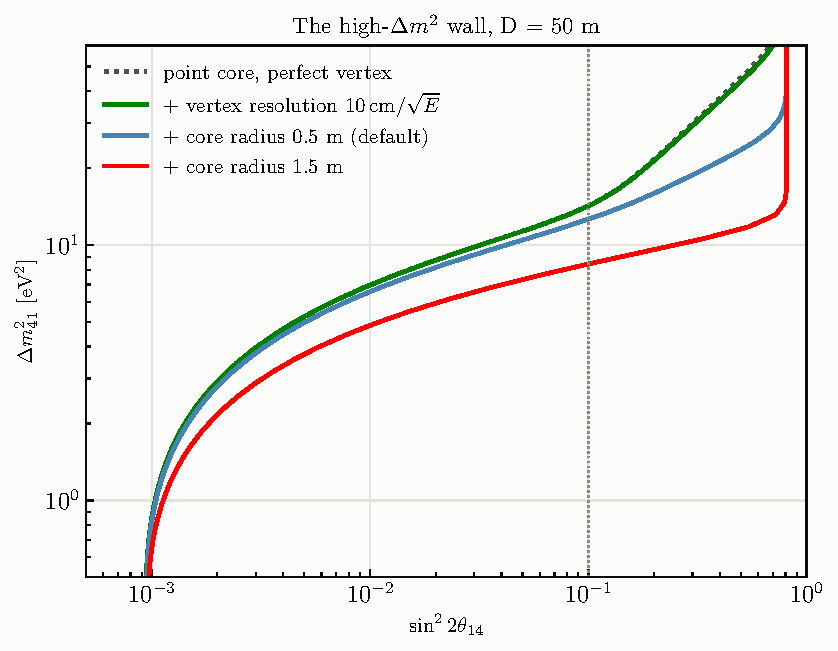
\includegraphics[width=\textwidth]{nb6_high_dm2_wall}
\caption{The high-$\dm{}$ wall dissected: idealised point source and perfect vertexing,
then the vertex resolution, then finite cores of $0.5$ and $1.5$~m.  The dotted vertical
line is $\st{14}=0.1$.  Every configuration loses sensitivity above its wall rather than
saturating, because a fully averaged depletion is degenerate with the free normalisation.}
\label{fig:wall}
\end{figure}

\begin{table}[t]\centering
\begin{tabular}{lccccc}\toprule
& $D=50$~m & 100~m & 200~m & 500~m & 1400~m\\\midrule
IBD rate [day$^{-1}$] & $6.1\times10^4$ & $1.5\times10^4$ & $3.7\times10^3$ & $590$ & $71$\\
baseline span [m] & $34$--$66$ & $84$--$116$ & $184$--$216$ & $484$--$516$ & $1384$--$1416$\\
best $\st{14}$ ($95\%$) & $9.5\times10^{-4}$ & $2.1\times10^{-3}$ & $5.0\times10^{-3}$ &
$2.2\times10^{-2}$ & $1.8\times10^{-1}$\\
at $\dm{41}$ [eV$^2$] & $0.50$ & $0.38$ & $0.29$ & $0.16$ & $0.065$\\
within $30\%$ over & $0.20$--$1.5$ & $0.17$--$0.87$ & $0.14$--$0.55$ & $0.08$--$0.30$ &
$0.03$--$0.12$\\
\bottomrule\end{tabular}
\caption{Sterile reach per standoff, $27\,\MWyr$ each.  Each standoff owns roughly a decade
of $\dm{}$ (the reach follows the accumulated phase $\Delta_{41}\propto\dm{}D/E$) while
the rate falls as $1/D^2$, so the compact standoffs carry the sensitivity and the
kilometre one buys only reach in $\dm{}$.}
\label{tab:sterile}
\end{table}

The findings, in order of importance:
\begin{itemize}\itemsep2pt
\item The vertex-binned search reaches $\st{14}=9.5\times10^{-4}$ at
$\dm{}=0.5\,\mathrm{eV^2}$, stays below $1.1\times10^{-3}$ over
$0.26$--$1.1\,\mathrm{eV^2}$ and below $2\times10^{-3}$ from $0.13$ to
$2.7\,\mathrm{eV^2}$: an order of magnitude beyond
the reactor short-baseline experiments, and covering the Gallium $2\sigma$ islands (which
span $0.8$--$10\,\mathrm{eV^2}$) in full.
\item \emph{An integrated analysis of the same data, with the same free flux shape, has no
sensitivity at all.}  One free mode per $E$ bin and a single $L$ bin leaves nothing to fit,
and its curve sits at $\st{14}\approx0.5$--$0.8$ over the whole range where the
$L$-binned search has reach, rising further at the edges (\cref{fig:lbin}).  The only integrated analysis with any reach is one that imposes the
Daya Bay flux shape --- the measurement that would itself have carried the depletion --- and
the vertex-binned search beats \emph{that} by $\sim3$--$4$ at its sweet spot near
$1$--$3\,\mathrm{eV^2}$, where its surviving $E$-wiggles resist the flux covariance, and by
up to $\sim90$ elsewhere.  Above $\sim15\,\mathrm{eV^2}$ the ordering reverses, since the
$L$-wiggle is smeared out while the $E$-wiggle is not.  So the finite detector is not an
improvement on the conventional analysis; it is what makes a prior-free search possible at
all.
\item Each standoff owns roughly a decade of $\dm{}$ (\cref{tab:sterile}).  The compact
standoffs are where the sensitivity is: $500$~m reaches $2\times10^{-2}$ and $1400$~m only
$1.8\times10^{-1}$, the $1/D^2$ rate cost outrunning the extra phase.  The full 3+1
formula matters at the few-percent level in the limit at $1.4$~km for
$\dm{}\lesssim0.1\,\mathrm{eV^2}$ --- the $\Delta_{34}$ term dilutes the wiggle, and the
$(1-s_{14})^2$ term of \cref{eq:wtemplate} adds $\sim3\%$ --- and is identically null at
50~m.
\item The high-$\dm{}$ wall is the \emph{energy} resolution, through the $L/E$ phase
($\sigma_\phi\propto\dm{}L\sigma_E/E^2$).  Quoting the $\dm{}$ at which the reach crosses
$\st{14}=0.1$: an idealised point source with perfect vertexing gives up at
$14\,\mathrm{eV^2}$, JUNO's vertexing costs almost nothing on top of that ($13$), and the
core size is the secondary effect --- $12\,\mathrm{eV^2}$ for a $0.5$~m core, $8$ for
$1.5$~m.  Compactness helps, but the energy resolution sets the ceiling.  Above the wall
every configuration loses sensitivity entirely, as it must: a fully averaged depletion is
$L$- and $E$-independent and is therefore exactly the normalisation this analysis leaves
free.
\item What limits the reach is statistics and the shape-only construction, not the
detector.  Freeing the reactor $E$-shape costs a factor $2.4$ against a pure-statistics
fit --- that is the price of not using the Daya Bay measurement, and it is worth paying ---
while the two response-uniformity fields together cost under $1\%$.  \eves{} rides along
but adds little: without $E_\nu$ reconstruction its wiggles wash out (the true-$T$ ratio
varies by $0.027$ peak-to-peak against $0.10$ in the input).
\end{itemize}

%======================================================================
\section{Axion-like particles from the core (notebook 7)}
\label{sec:alps}

\subsection{Physics and formalism}
\label{sec:alp_formalism}
The core is a photon source of $\sim5\times10^{18}\,\gamma/\mathrm{s}$: photons scattering
in the fuel convert to ALPs by Primakoff ($g_{a\gamma\gamma}$, coherent $Z^2$ on uranium) or
Compton-like ($g_{aee}$) processes, stream unimpeded through shielding, and reach JUNO,
where they scatter back into visible photons or electrons through the inverse processes or
decay in flight.  I follow the calculation of Ref.~\cite{AristizabalSierra:2025myf} for
liquid-scintillator detectors, with the underlying formulas of
Refs.~\cite{AristizabalSierra:2020rom,Dent:2019ueq}; every expression below is the one
implemented in \texttt{reactor/alps.py}.  The Lagrangian is
$\mathcal L\supset-\tfrac14g_{a\gamma\gamma}\,aF_{\mu\nu}\tilde F^{\mu\nu}-ig_{aee}\,a\,\bar e\gamma_5e$,
and one coupling is switched on at a time.

\paragraph{Reactor photon flux.}
The prompt continuum is the FRJ-1 power law \cite{Bechteler:1984,AristizabalSierra:2020rom}
\begin{equation}
\frac{d\Phi_\gamma}{dE_\gamma}=5.8\times10^{17}\Big(\frac{P}{\mathrm{MW}}\Big)
e^{-1.1E_\gamma/\mathrm{MeV}}\ \mathrm{MeV^{-1}s^{-1}},
\label{eq:flux}
\end{equation}
which integrates to $1.75\times10^{18}\,\gamma/\mathrm{s}$ above 1~MeV at $10\,\mathrm{MW}$
(the analytic $5.8\times10^{18}e^{-1.1}/1.1$).  MINER's simulated flux is $\sim20\times$
larger, so \cref{eq:flux} is the conservative choice, and the one made by the reference
analyses.

\paragraph{Primakoff production and inverse-Primakoff detection.}
For $\gamma(p_1)+N(p_2)\to a(k_1)+N(k_2)$ on a nucleus of mass $M$, charge $Z$, the exact
$2\to2$ cross section \cite{Aloni:2019ruo,AristizabalSierra:2020rom} is
\begin{equation}
\frac{d\sigma_P}{dt}=2\alpha Z^2F^2(t)\,g_{a\gamma\gamma}^2\,
\frac{M^4}{t^2(M^2-s)^2(t-4M^2)^2}
\Big\{m_a^2t\,(M^2+s)-m_a^4M^2-t\big[(M^2-s)^2+st\big]\Big\},
\label{eq:primakoff}
\end{equation}
integrated over $t\in[t_{\min},t_{\max}]$, $t_{\max/\min}=m_a^4/4s-(p_{1\rm cm}\mp k_{1\rm cm})^2$
with $p_{1\rm cm}=(s-M^2)/2\sqrt s$, $k_{1\rm cm}=[(s+m_a^2-M^2)^2/4s-m_a^2]^{1/2}$,
$s=M^2+2ME_\gamma$, on a logarithmic $t$-grid (the integrand is sharply forward-peaked).
The atomic screening form factor is the Thomas--Fermi--Moli\`ere form
$F^2(t)=[a_0^2|t|/(1+a_0^2|t|)]^2$, $a_0=184.15\,e^{-1/2}/(Z^{1/3}m_e)$, essential below
$m_a\sim10$~keV; the nuclear form factor is negligible for $E_a\lesssim10$~MeV.  Because
$|t|/M^2\ll1$ the ALP carries the photon energy, $E_a\simeq E_\gamma$, so the emitted flux is
\begin{equation}
\frac{d\Phi_a}{dE_a}=\frac{\sigma_P(E_a)}{\sigma_{\rm SM}(E_a)}\,
\frac{d\Phi_\gamma}{dE_\gamma}\Big|_{E_\gamma=E_a},
\label{eq:alpflux}
\end{equation}
where $\sigma_{\rm SM}$ (Rayleigh + Compton + photoelectric + pair) is the total photon
cross section in uranium from XCOM \cite{XCOM}; the branching ratio
$\sigma_P/(\sigma_P+\sigma_{\rm SM})$ is $\sigma_P/\sigma_{\rm SM}$ to excellent accuracy in
the coupling range of interest.  Detection by inverse Primakoff on carbon and hydrogen uses
$\sigma_P^{\rm det}=2\sigma_P$ (spin counting: a spin-0 initial state instead of spin-1).

\paragraph{Compton-like production and inverse-Compton detection.}
For $\gamma e\to ae$ with $s=m_e^2+2E_\gamma m_e$, threshold $s>(m_a+m_e)^2$ i.e.\
$E_\gamma^{\rm th}=m_a+m_a^2/2m_e$, and $x=1-E_a/E_\gamma+m_a^2/2E_\gamma m_e$
\cite{Brodsky:1986mi,AristizabalSierra:2020rom}:
\begin{equation}
\frac{d\sigma_C}{dx}=\frac{\alpha g_{aee}^2\,x}{4(s-m_e^2)(1-x)}
\Big[x-\frac{2m_a^2s}{(s-m_e^2)^2}+\frac{2m_a^2}{(s-m_e^2)^2}
\Big(\frac{m_e^2}{1-x}+\frac{m_a^2}{x}\Big)\Big],
\label{eq:compton}
\end{equation}
integrated over $x_{\min,\max}=\big[(s-m_e^2)(s-m_e^2+m_a^2)\mp(s-m_e^2)
\sqrt{(s-m_e^2+m_a^2)^2-4sm_a^2}\big]/2s(s-m_e^2)$; the ALP flux is the convolution of
$\sigma_C^{-1}d\sigma_C/dE_a\times\sigma_C/\sigma_{\rm SM}$ with the photon flux
(Ref.~\cite{AristizabalSierra:2025myf}, Eq.~14).  Detection by inverse Compton
$ae\to\gamma e$ uses (Ref.~\cite{AristizabalSierra:2025myf}, Eq.~22)
\begin{equation}
\frac{d\sigma_{IC}}{dE_\gamma}=\frac{\alpha g_{aee}^2}{32\pi}\,\frac{y}{m_e^2p_a^2E_\gamma}
\Big(1+\frac{4m_e^2E_\gamma^2}{y^2}-\frac{4m_eE_\gamma}{y}
-\frac{4m_a^2m_ep_a^2E_\gamma\sin^2\theta}{y^3}\Big),\qquad y=2m_eE_a+m_a^2,
\label{eq:invcompton}
\end{equation}
integrated over $E_\gamma\in[y/2(m_e+E_a+p_a),\,y/2(m_e+E_a-p_a)]$ with
$\cos\theta=(m_e+E_a-y/2E_\gamma)/p_a$.  Axio-electric absorption is neglected: it scales
as $Z^5$ and on carbon at MeV energies is $\sim10^{-4}$ of the germanium rates of the
reference analyses, negligible against inverse Compton here.

\paragraph{Decays, survival and decay-in-detector probabilities.}
\begin{equation}
\Gamma(a\to\gamma\gamma)=\frac{g_{a\gamma\gamma}^2m_a^3}{64\pi},\qquad
\Gamma(a\to e^+e^-)=\frac{g_{aee}^2m_a}{8\pi}\sqrt{1-\frac{4m_e^2}{m_a^2}}\ \ (m_a>2m_e),
\label{eq:widths}
\end{equation}
with lab decay length $\ell_a=(p_a/m_a)\,\hbar c/\Gamma_a$.  An ALP produced in the core
survives to the detector centre with $P_{\rm surv}=e^{-L/\ell_a}$ (for scattering,
evaluated at $L=D=50$~m) or to the front face with $e^{-(D-R)/\ell_a}$, and then decays
inside with probability
\begin{equation}
P_{\rm decay}=1-\exp\!\big(-\bar\ell/\ell_a\big),\qquad \bar\ell=\tfrac43R=22\,\mathrm{m},
\label{eq:pdecay}
\end{equation}
the mean chord of the fiducial sphere (this replaces the fixed depth $r=0.7$~m of the
JUNO-TAO geometry).  The decay-length boundary of Ref.~\cite{AristizabalSierra:2025myf},
Eq.~(53), corrected to $g^2=8\pi\hbar c/(Lm_a\beta)$, is reproduced numerically to
$10^{-4}$.

\paragraph{Event yields.}
Over a live time $\Delta t$ (27~MW\,yr $=$ 3~yr at $90\%$ duty), with $\mathcal A=\pi R^2=
855\,\mathrm{m^2}$ the detector face and $N_{C,H,e}$ the fiducial target counts,
\begin{align}
N_{\rm scat}^{P}&=\frac{\Delta t}{4\pi D^2}\int dE_a\,\frac{d\Phi_a}{dE_a}\,e^{-D/\ell_a}\,
2\big[N_C\sigma_P^{C}(E_a)+N_H\sigma_P^{H}(E_a)\big],\\
N_{\rm scat}^{IC}&=\frac{\Delta t}{4\pi D^2}\int dE_a\,\frac{d\Phi_a}{dE_a}\,e^{-D/\ell_a}\,
N_e\,\sigma_{IC}(E_a),\\
N_{\rm decay}&=\frac{\mathcal A\,\Delta t}{4\pi D^2}\int dE_a\,\frac{d\Phi_a}{dE_a}\,
e^{-(D-R)/\ell_a}\,\big[1-e^{-\bar\ell/\ell_a}\big],
\label{eq:yields}
\end{align}
with $E_a$ integrated over the single-hit window $3$--$10$~MeV.  Compared with JUNO-TAO we
trade a GW reactor for $10\,\mathrm{MW}$ and 30~m for 50~m, but gain $\sim2\times10^4\times$
the target mass and $\sim25\times$ the decay path; the decay term \eqref{eq:yields} is what
carries the reach.

\paragraph{Validation.}
I checked every ingredient.  $\Gamma(a\to\gamma\gamma)$ and $\Gamma(a\to e^+e^-)$ agree with
analytic evaluation to $10^{-4}$ and vanish below the $e^+e^-$ threshold.  The exact
Primakoff form \eqref{eq:primakoff} agrees with an independent implementation of the Dent
et al.\ forward/recoilless form ($d\sigma/d\cos\theta=\tfrac14g^2\alpha Z^2F^2|\vec p_a|^4
\sin^2\theta/t^2$) at the $6$--$40\%$ level, with the largest deviations near threshold and at
high energy, which is exactly the deviation Ref.~\cite{AristizabalSierra:2020rom}
(footnote~5) reports for that approximation.  The Compton cross section has the right
threshold and positivity, and the right magnitude ($\alpha g^2/m_e^2$, i.e.\ of order
Klein--Nishina at $g_{aee}=1$: $3.3\times10^{-25}$ against
$2.1\times10^{-25}\,\mathrm{cm^2}$ at 1~MeV).  The uranium $\sigma_{\rm SM}$ reproduces its
XCOM anchors, and the flux integral its analytic value.

\paragraph{Background and statistics.}
The single-hit window is $3$--$10$~MeV.  The background is our own model of \cref{sec:sm}:
reactor \eves{} $3.3\times10^5$, IBD singles $3.6\times10^5$ and solar \eves{}
$3.1\times10^4$ events over the exposure ($7.3\times10^5$ in total).  Cosmogenics ($^{12}$B
and friends) are not modelled; since $\chi^2\propto g^8/N_b$, the reach in the coupling
scales only as $N_b^{1/8}$, and even a $4\times$ larger background costs $20\%$.  Following
Ref.~\cite{AristizabalSierra:2025myf}, Eq.~(54), the single-bin statistic is
$\chi^2=N_s^2/(N_s+N_b+\sigma_{\rm sys}^2N_s^2)$ with $\sigma_{\rm sys}=0.1$, and $90\%$~CL
is $\Delta\chi^2=4.61$ (2 dof).  The background-free limit is shown alongside, since the
prompt/delayed photon and vertex handles of a LS detector could approach it.

\subsection{Results}
\begin{figure}[t]\centering
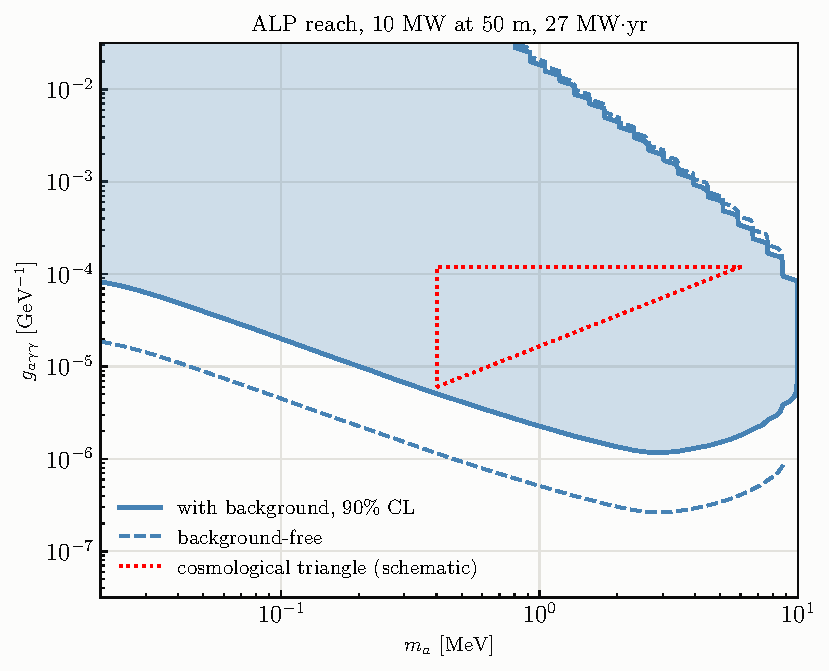
\includegraphics[width=\textwidth]{nb7_alp_photon}
\caption{$90\%$~CL exclusion in the ALP--photon plane for $27\,\MWyr$, with the full
background (solid, filled) and background-free (dashed).  The dotted wedge is the
schematic cosmological triangle of Ref.~\cite{AristizabalSierra:2020rom}, Fig.~10.}
\label{fig:alp_photon}
\end{figure}
\begin{figure}[t]\centering
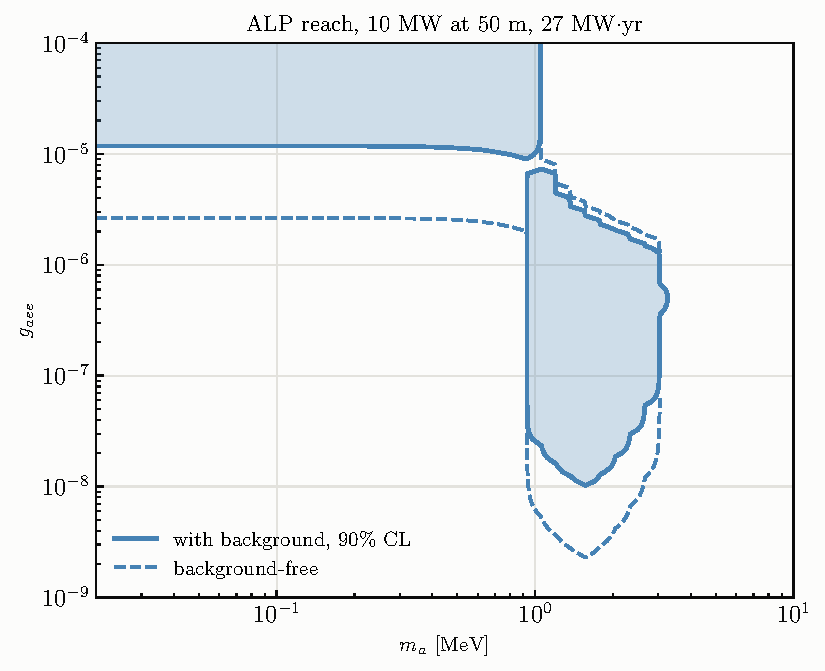
\includegraphics[width=\textwidth]{nb7_alp_electron}
\caption{Same in the ALP--electron plane; above the $e^+e^-$ threshold the decay channel
opens the band down to $g_{aee}\sim10^{-8}$.}
\label{fig:alp_electron}
\end{figure}

The decay channel dominates by orders of magnitude at MeV masses (\cref{fig:alp_photon}):
at $m_a=1$~MeV and $g_{a\gamma\gamma}=10^{-5}\,\mathrm{GeV^{-1}}$ there are $7\times10^5$
decays against $0.06$ scatterings over the exposure.  With the background included, at
$m_a=1$~MeV the excluded band is
$g_{a\gamma\gamma}\in[2.3\times10^{-6},\ 1.4\times10^{-2}]\,\mathrm{GeV^{-1}}$, so the
schematic cosmological triangle, the wedge at $m_a\sim0.3$--$5$~MeV and
$g_{a\gamma\gamma}\sim10^{-5}$--$10^{-4}\,\mathrm{GeV^{-1}}$ between the beam-dump, HB-star
and SN1987A exclusions where only cosmology-dependent bounds apply
\cite{Depta:2020wmr,Jaeckel:2006xm}, is covered in full.  For scale, JUNO-TAO with
background reaches $g\sim$~few$\times10^{-4}$ \cite{AristizabalSierra:2025myf}; the
near-reactor plus JUNO combination goes an order of magnitude deeper at the same reactor-off
cost.  In the electron plane (\cref{fig:alp_electron}), at $m_a=1.5$~MeV the excluded band
is $g_{aee}\in[1.2\times10^{-8},\ 3.1\times10^{-6}]$ with background, so the unexplored
stripe that Ref.~\cite{AristizabalSierra:2025myf} identifies is reached without the
background-free assumption TAO needs.  The caveats are the FRJ-1 flux, the absence of
cosmogenics, single-bin counting (an energy-shape fit would only help), the pure-uranium
core, the neglect of ALP attenuation in the shielding, and the schematic triangle overlay.

%======================================================================
\section{Discussion and caveats}
\label{sec:discussion}

The three studies share a lesson about what a parked reactor's \emph{size and proximity}
do for a 20~kt detector.  For the SM couplings the win is the IBD anchor: $20\times$ the
\eves{} statistics with the \emph{same} flux, cancelling normalisation, flux shape and
energy response against a transfer budget of a few tenths of a percent.  For sterile oscillations the win is
the detector's finite size, which converts the oscillation into an $L$-direction
observable that no source systematic can mimic, and which crucially allows a shape-only
analysis independent of the Daya Bay measurement that would otherwise carry the signal.  For
ALPs the win is the decay volume: an $855\,\mathrm{m^2}$ face and a 22~m chord watching a
$5\times10^{18}\,\gamma/\mathrm{s}$ source.

The stated caveats are real.  The detector singles are subtracted with reactor-off
running (\cref{sec:singles}), but their spectral shape is a component model
rather than a transport simulation and the cosmogenic rates are depth-scaled estimates;
what protects the result is that it depends on them only through $\sqrt{B}$.  They are
still unmodelled in the ALP window, where they would enter the reach as $N_b^{1/8}$ and
cost a few percent.  The reactor spectrum is undefined below the IBD threshold, which is
where $48\%$ of the \eves{} window rate sits; that costs the answer nothing, but it means
the quoted \eves{} rate is a lower bound.  The transfer budget of \cref{sec:sm} is
essentially the whole of the weak-mixing-angle result, and its leading term ---
$N_e/N_p$ times the relative selection efficiency, assumed to $0.5\%$ --- is not a neutrino
measurement but a scintillator-composition one, which is where the effort belongs.  The two
response-uniformity fields of the sterile search ($0.5\%$ efficiency and $0.2\%$ energy
scale over the volume) are assumptions that should be replaced by JUNO's calibration
numbers, though that search turns out not to be limited by them.  A companion feasibility estimate (notebook 8)
finds that the reactor's own neutron and gamma leakage require a research-reactor-class
shield ($\sim6$~m water-equivalent, or $\sim2$~m steel plus a sub-metre high-$Z$ collar, on
top of JUNO's 4~m of pool water) for the near-reactor programme not to spoil single-hit
physics; this is exactly what a TRIGA-style pool installation provides.  Finally, the
mobile-reactor $\theta_{13}$ study (notebook 2) remains the strongest oscillation argument
for such a source: the fixed-reactor variant (notebook 2b) shows that the 33~m detector
provides only $0.026$~rad of $\theta_{13}$ phase and cannot substitute for moving the source.
The same finite size that is the right tool at metre oscillation lengths is the wrong one at
kilometres.

\appendix

\section{Daya Bay flux model and covariance}
\label{app:flux}

\paragraph{The measured spectra.}
Daya Bay's unfolding \cite{DayaBay:2021dqj} releases the per-fission IBD yields
$\Phi^0_i$ [$\mathrm{cm^2\,fission^{-1}}$] in $n=25$ neutrino-energy bins of width
$0.25$~MeV over $E_\nu\in[1.8,\,8.0]$~MeV, for three spectra ($^{235}$U, $^{239}$Pu, and
the ``Total'', their cycle-averaged mixture at fission fractions
$0.564:0.076:0.304:0.056$), with a $75\times75$ covariance $V$ over the stacked
$[\,^{235}\mathrm{U},\,^{239}\mathrm{Pu},\,\mathrm{Total}\,]$ vector.  The near-reactor
studies of this report use the $^{235}$U yields with the $25\times25$ block, which is the
only measured shape uncertainty they carry: the $^{239}$Pu component is $6.3\%$ of fissions
at mid-cycle and $12.5\%$ at end of cycle, and its shape freedom is represented by the
$\pm30\%$ fuel-evolution mode of \cref{eq:evomode} rather than by its own covariance block.
The standard JUNO analysis (below) uses the Total.

\Cref{fig:dyb_iso} shows the measured $^{235}$U and $^{239}$Pu yields with their released
$1\sigma$ uncertainties (the diagonal of $V$; the last bin spans $7.8$--$9.5$~MeV),
converted into IBD rates at JUNO for a hypothetical pure 10~MW core of each isotope at
50~m, together with the Huber--Mueller $^{238}$U and $^{241}$Pu spectra used for the
minority components.  The Huber--Mueller polynomial fits are valid only up to $8.5$~MeV;
above it the code applies an artificial exponential cutoff (marked in the figure), which is
why the $^{238}$U and $^{241}$Pu curves kink there.  This is immaterial, since these are
$1$--$2\%$ components and contribute nothing to any analysis above 8~MeV.
\Cref{fig:haleu_cycle} is the companion: the actual HALEU core at the start ($\beta=0$),
middle and end ($\beta=1$) of its cycle, built from those ingredients through
\cref{eq:source,eq:evolution}, with a $5\%$ rate drop and a slight softening
($2.00\to1.90\times10^7$ IBD per year); its bottom panel shows the shape change as a ratio
to the start of cycle.  \Cref{fig:leu_cycle} is the same figure for a commercial-LEU core,
the Daya Bay measured fission fractions across their cycle ($F_{235}=0.66\to0.49$,
$F_{239}=0.23\to0.36$), at the same power and distance.  The LEU core has a $5\%$ lower
absolute rate (plutonium-rich fuel yields fewer $\bar\nu_e$ per unit power), and because
the HALEU model applies Daya Bay's Pu \emph{increments} on top of a $^{235}$U-dominated
fresh core, its end-of-cycle distortion ($\sim10\%$ at 8~MeV) is essentially the LEU one.
That is the statement ``follows the Daya Bay trajectory'' made visible, and the reason it
is a conservative model for a $2\%$-$^{238}$U core, whose real plutonium breeding is slower.

\begin{figure}[t]\centering
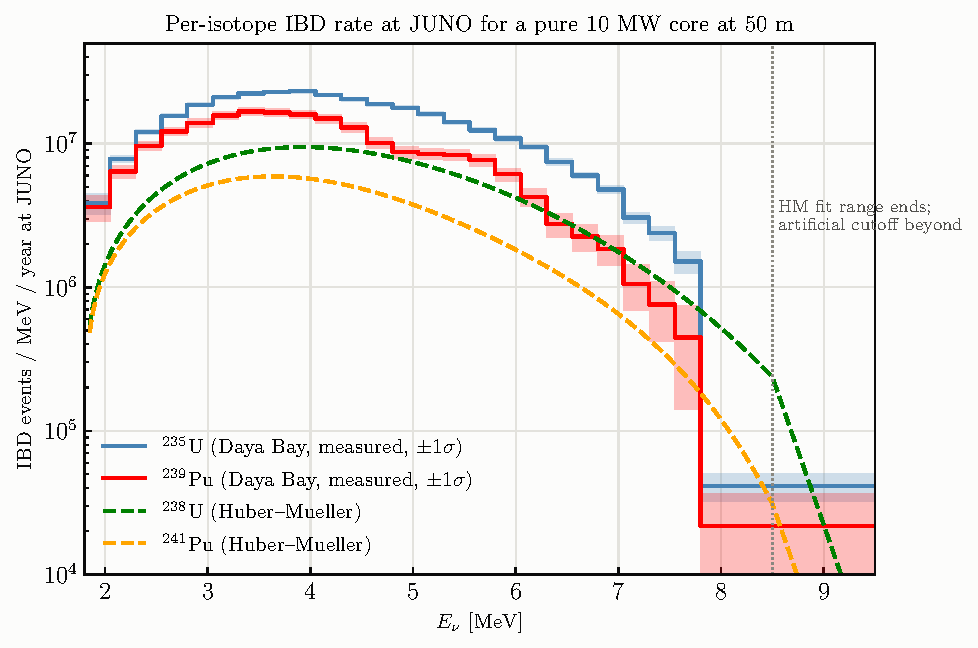
\includegraphics[width=\textwidth]{appA_dayabay_isotopes}
\caption{Per-isotope IBD rate at JUNO for a pure 10~MW core of each isotope at 50~m:
the measured Daya Bay $^{235}$U and $^{239}$Pu yields \cite{DayaBay:2021dqj} with their
released $1\sigma$ uncertainties as bands, and the Huber--Mueller
\cite{Huber:2011wv,Mueller:2011nm} $^{238}$U and $^{241}$Pu spectra (dashed).  The dotted
line marks the end of the Huber--Mueller fit range.}
\label{fig:dyb_iso}
\end{figure}
\begin{figure}[t]\centering
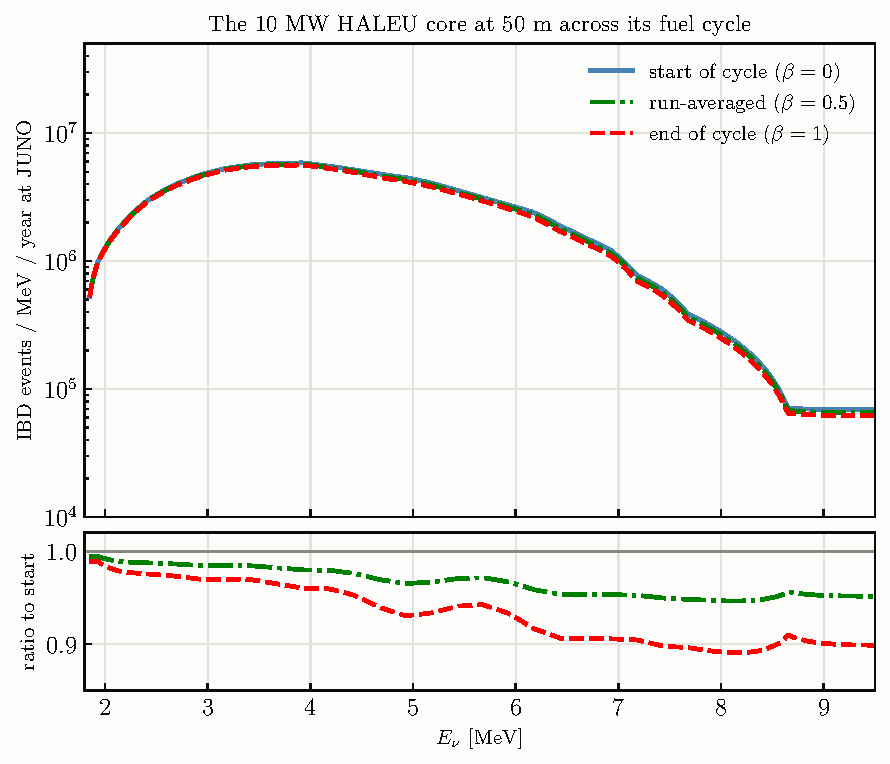
\includegraphics[width=\textwidth]{appA_haleu_cycle}
\caption{The 10~MW HALEU core at 50~m at start, middle and end of its fuel cycle
(\cref{eq:evolution}), built from the spectra of \cref{fig:dyb_iso}; bottom: ratio to the
start of cycle.}
\label{fig:haleu_cycle}
\end{figure}
\begin{figure}[t]\centering
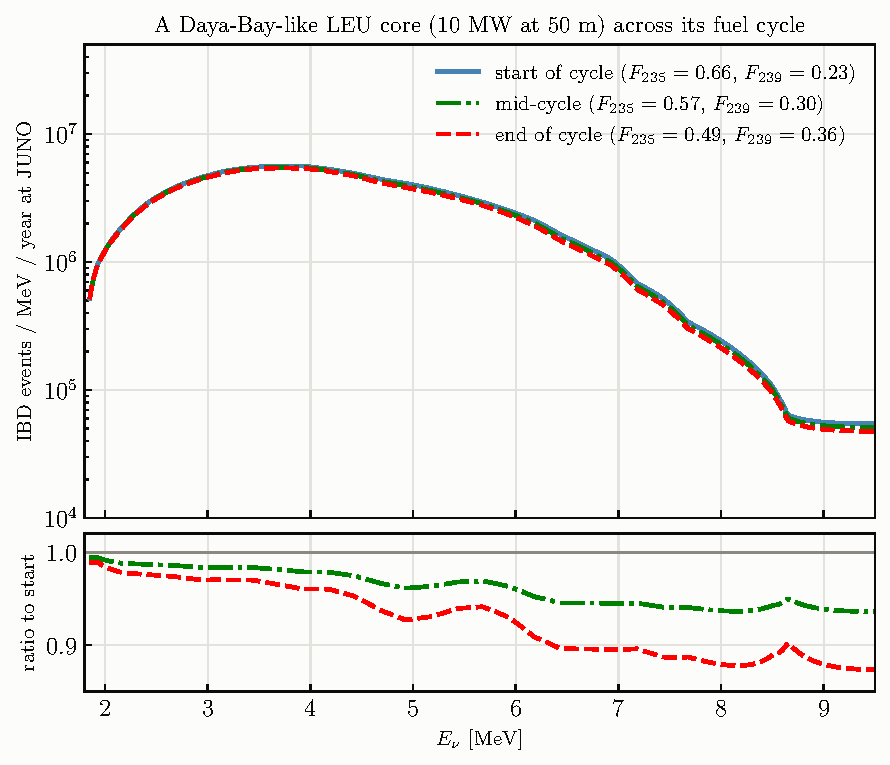
\includegraphics[width=\textwidth]{appA_leu_cycle}
\caption{Same for a commercial-LEU core: the Daya Bay measured fission fractions
\cite{DayaBay:2017jkb} at the start, middle and end of their 20 burnup groups, at the same
10~MW and 50~m so the two figures are directly comparable.}
\label{fig:leu_cycle}
\end{figure}

\paragraph{From binned yields to a continuous flux (the NuFit prescription).}
Following Appendix~A of the NuFit analysis that the repository's standard method
reproduces, the continuous flux times cross section is written as a smooth reference shape
times a modulation,
\begin{equation}
S(E)=\phi_{\rm HM}(E)\,\sigma_{\rm IBD}(E)\;\sum_{m=1}^{n}y_m\,\delta_m(E),
\label{eq:appA_shape}
\end{equation}
where $\phi_{\rm HM}$ is the Huber--Mueller spectrum at the Daya Bay average fission
fractions (with no isotope correction), $\sigma_{\rm IBD}$ is Vogel--Beacom, and
$\{\delta_m\}$ are the cardinal cubic splines through the 25 bin centres
($\delta_m(E_{m'})=\delta_{mm'}$).  The coefficients are fixed by demanding that the
bin-averaged prediction reproduce the measured yields exactly:
\begin{equation}
M_{im}=\frac{1}{\Delta E_i}\int_{\rm bin\,i}\phi_{\rm HM}\sigma_{\rm IBD}\,\delta_m\,dE,\qquad
\bm y^0=M^{-1}\bm\Phi^0,
\label{eq:appA_M}
\end{equation}
with the integrals done on a dedicated 1~keV grid; the residual
$\max_i|(M\bm y^0)_i-\Phi^0_i|/\Phi^0_i$ is $6\times10^{-16}$.  Above the last measured
bin ($9.5$~MeV after the release's extension) the modulation is held constant.

\paragraph{From covariance to pulls.}
The covariance is recast as $n$ unit-Gaussian pulls by eigendecomposition,
$V=O\,D\,O^T$, $\Psi=O\sqrt D$ (columns are modes), and each mode is pushed through the
same interpolation, $\bm y^{(k)}=M^{-1}\Psi_{\cdot k}$, so that a pull $\xi_k$ distorts
the flux by
\begin{equation}
S(E)\;\to\;S(E)\Big[1+\sum_k\xi_k\,\frac{\sum_ny^{(k)}_n\delta_n(E)}{\sum_ny^0_n\delta_n(E)}\Big],
\qquad \chi^2\supset\sum_k\xi_k^2,
\label{eq:appA_pulls}
\end{equation}
which is exact to first order and keeps the pull penalty diagonal.  In the near-reactor
modules the same construction is applied to the relative covariance
$V_{ij}/(\Phi^0_i\Phi^0_j)$ of the $^{235}$U block, and in the joint fit of \cref{sec:sm}
each of the 25 modes acts on the IBD anchor and the \eves{} spectrum \emph{coherently},
which is what lets the anchor measure it away; the modes are then interpolated linearly in
$E$ and enter the Asimov covariance $C=\mathrm{diag}(\mu)+\sum_kv_kv_k^T$ as $v_k=t\,\partial\mu/\partial\xi_k$.
Modes with eigenvalue below $10^{-10}$ of the largest are dropped.  In the sterile analysis
of \cref{sec:sterile} this prior is deliberately \emph{not} used, and the flux shape and
normalisation are left free, for the reason explained there.

\paragraph{The measured Total flux and JUNO's own spectrum.}
For the standard far-reactor analysis, the NuFit prescription additionally rescales the
prediction bin-per-bin to JUNO's recovered un-oscillated spectrum,
\begin{equation}
k_i=\frac{\big(N^{\rm obs}_i-B_i\big)/\overline{P}_{ee,i}}{N^{\rm pred,unosc}_i},
\label{eq:binscale}
\end{equation}
where $\overline{P}_{ee,i}$ is JUNO's own released model survival probability per bin;
this pins the un-oscillated shape to data and turns flux-model and cross-section choices
into nulls (it was found to be the decisive ingredient in reproducing JUNO's solar-parameter
result to $0.06\sigma$).  It has no analogue for projections, where the measured flux with
its covariance takes its place.

\section{Systematics of the standard JUNO analysis (NuFit procedure)}
\label{app:nufit}

The repository's standard far-reactor analysis reproduces the NuFit 6.1 treatment of the
JUNO 59.1-day data \cite{JUNO:2025gmd}, and its nuisance set is what the near-reactor
studies inherit for the far side and for the detector response.  The test statistic is
\begin{equation}
\chi^2=\sum_i\frac{\big(N^{\rm obs}_i-N^{\rm pred}_i(\bm\xi)\big)^2}{\sigma^2_{{\rm CNP},i}}
+\sum_a\Big(\frac{\xi_a}{\sigma_a}\Big)^2,\qquad
\frac{3}{\sigma^2_{{\rm CNP},i}}=\frac{1}{N^{\rm obs}_i}+\frac{2}{N^{\rm pred}_i},
\label{eq:chi2}
\end{equation}
the combined Neyman--Pearson form used by JUNO (NuFit's own default is the Poisson
Baker--Cousins form $2\sum_i[P_i-O_i+O_i\ln(O_i/P_i)]$; the two agree to $10^{-4}$ in
$\sin^2\theta_{12}$).  The prediction is
\begin{equation}
N^{\rm pred}_i=(1+\xi_{\rm norm})\,k_i\,\mathcal N\sum_{\rm cores\,c}\Big[R\big(\xi_{\rm scl},\xi_{\rm bias},\xi_{\rm res}\big)\;
S\big(E;\{\xi_k\}\big)\,\frac{P_{ee}(E,L_c)}{4\pi L_c^2}\Big]_i+\sum_bB_{b,i}\,(1+\xi_b)\,(1+\delta_{b,{\rm LiHe}}\,\xi_{\rm sh}E_i),
\label{eq:pred}
\end{equation}
with the nine signal cores (Yangjiang, Taishan and the effective Daya Bay core at 215~km),
matter effects at $2.55\,\mathrm{g\,cm^{-3}}$, and the response
\begin{equation}
\tilde E_{\rm pr}=E_{\rm pr}\,r_{\rm nl}\big[(1+\xi_{\rm scl})F_{\rm nl}(E_{\rm pr})+\xi_{\rm bias}\big],\qquad
\sigma(\tilde E)=(1+\xi_{\rm res})\,r_{\rm res}\,\sqrt{a^2\tilde E+b^2\tilde E^2},
\label{eq:response}
\end{equation}
$F_{\rm nl}$ being JUNO's released positron non-linearity and $a=3.3\%$, $b=1.0\%$.
\Cref{tab:nufit} lists every pull and its prior in the standard configuration.

\begin{table}[t]\centering
\begin{tabular}{llc}\toprule
pull & meaning & prior $\sigma$\\\midrule
$\xi_{\rm norm}$ & signal normalisation & $2.4\%$ = $1.8\%$ (Tab.~2 rates) $\oplus$ $1.6\%$ (selection efficiency)\\
$\xi_{\rm scl}$ & energy scale & $0.5\%$\\
$\xi_{\rm bias}$ & energy bias (offset in $F_{\rm nl}$ units) & $0.5\%$\\
$\xi_{\rm res}$ & resolution & $5\%$\\
$\xi_{\rm LiHe}$ & $^9$Li/$^8$He normalisation & $33\%$\\
$\xi_{\rm sh}$ & $^9$Li/$^8$He linear-in-$E$ shape (20\% at 1~MeV) & $0.20$\\
$\xi_{\rm geo}$ & geoneutrino normalisation & $42\%$\\
$\xi_{\rm world}$ & world-reactor normalisation & $10\%$\\
$\xi_{\rm BiPo}$ & $^{214}$Bi--$^{214}$Po normalisation & $56\%$\\
$\xi_{\rm other}$ & other backgrounds & $100\%$\\
$\xi_k$, $k=1..25$ & Daya Bay flux-shape modes (\cref{app:flux}) & $1$ each\\\midrule
$r_{\rm BG}$ & overall background rescaling (all but geoneutrinos) & fixed, $1.00$ (NuFit cnf~2: $1.15$)\\
$r_{\rm nl}$, $r_{\rm res}$ & non-linearity / resolution rescalings & fixed, $1.0$ (cnf~3: $1.024$; cnf~5: $1.3$)\\
\bottomrule\end{tabular}
\caption{Nuisance parameters of the standard analysis.  The $2.4\%$ normalisation is the
NuFit ``note added'' budget; their published Tab.~1 configurations use $1.8\%$.  External
inputs: $\sin^2\theta_{13}=0.02175$, $\dmee=2.466\times10^{-3}\,\mathrm{eV^2}$ (Daya Bay).}
\label{tab:nufit}
\end{table}

\paragraph{Profiling.}
The prediction is affine in the three energy pulls (through the response matrix) and the 25
flux pulls (through the spectrum) at fixed oscillation parameters, so a linear basis is
built once per grid point and the 28 pulls plus the background nuisances are profiled
analytically; the two oscillation parameters are minimised numerically.  In the Asimov
projections of \cref{sec:sm,sec:sterile} the same nuisances become the joint modes of
$C=\mathrm{diag}(\mu)+\sum_kv_kv_k^T$ and no minimisation is performed at all.

\paragraph{What the reproduction established.}
With this treatment the repository reproduces NuFit's Tab.~2 relative fluxes exactly, their
best fit to $0.10\sigma$, and their $\dmee$ profile; with the note-added budget it lands on
JUNO's official $(\sin^2\theta_{12},\dm{21})$ at $0.06\sigma$ with every nuisance well
inside its prior.  The decisive ingredients, in order, were including the Daya Bay complex
in the signal (its $\Delta_{21}\approx2\pi$ position fills the solar dip), the bin-per-bin
rescaling of \cref{eq:binscale}, and the $2.4\%$ normalisation.  The residual difference in
the ellipse tilt corresponds to about $3\%$ of effective rate freedom, that is, only
$\sqrt{3^2-2.4^2}\approx1.8\%$ beyond the documented budget, and it must be coherent in
energy (candidates: the delivered-power history, the absolute Daya Bay flux anchor, the
target proton count, and off-equilibrium/spent-fuel corrections).

\bibliographystyle{apsrev4-2}
\bibliography{ref}
\end{document}
